\typeout{NT FILE DESIGN.tex}%
\chapter{Design}%
\label{ch:design}
\begin{quote}
\begin{flushright}
``\emph{Simplicity is the ultimate sophistication.}'' \\
\textbf{-- Leonardo Da Vinci}, polymath
\end{flushright}
\end{quote}

Addressing the conflicting demands of security, safety, and \gls{swap-c}
efficiency in \glspl{uav} requires rethinking conventional mixed-criticality
architectures. This chapter presents the design of the \gls{sspfs}: a
trustworthy flight stack that leverages the Bao hypervisor for
video-surveillance applications, where resource-intensive but non-critical
streaming coexists with safety-critical flight control on consolidated hardware.

We begin by defining requirements and constraints for the target application,
then analyze the conventional architecture and identify its drawbacks. Next, we
integrate all components on a single platform without supervision: the
\gls{uspfs} baseline, used to assess consolidation and its performance
overhead. Finally, we run this baseline atop the Bao hypervisor, yielding the
\gls{sspfs}.

We then select the hardware -- the \gls{uav} and the \gls{uavic} -- and map these
components into the \gls{uspfs} and \gls{sspfs} systems. To support shared
\gls{pcie} devices across \glspl{vm}, we design a mailbox-supervision
mechanism. We conclude by adapting the hardware mapping to the constraints
imposed by the \gls{uavic} platform and Bao.

% The conventional \gls{umpfs} approach employs separate hardware nodes a flight controller for critical systems and a companion computer for tasks like collision avoidance or video streaming. While providing functional separation, this architecture increases weight and power consumption while offering no isolation guarantees, allowing compromises in the companion node to propagate to flight systems.

% Merging flight control and companion functions onto a single platform reduces weight, power requirements, and inter-component latency. However, unsupervised consolidation (\gls{uspfs}) introduces critical risks including performance interference (where non-critical tasks disrupt flight-critical operations) and security vulnerabilities (where a single compromise affects the entire system). Consequently, unsupervised consolidation alone cannot meet stringent safety and security requirements.

% The supervised approach hypothesizes that hypervisor oversight enables secure consolidation while preserving SWaP advantages. The \gls{sspfs} employs the Bao hypervisor to achieve hardware-enforced isolation between flight control and companion functions, certifiable separation with minimal performance overhead, and retention of single-board SWaP benefits. The following sections detail this architecture's requirements, components, and security model.

\section{Requirements and Constraints}
\label{sec:req-sec}
Video surveillance missions necessitate geolocation control to survey a
designated target area and image acquisition to gather pertinent information
about that region. Both objectives can be achieved through offline or online
command methods, or a combination of the two~\cite{gugan2023path}.
%
In the offline command approach, the target area and the specific information to
be captured are well-defined and can be comprehensively specified \emph{a
priori} to the \gls{uav}~\cite{gugan2023path}. For instance, in cartographic
applications, the \gls{uav} systematically scans the target area to collect
topographic data~\cite{caroti_uav-borne_2017}. Consequently,
the UAV can operate in a fully autonomous mode, with data being directly stored
in its onboard storage systems~\cite{qgc-survey}.

Conversely, the online command approach is more suitable for dynamic and
unpredictable environments, where the target area and relevant information are
not fully predefined~\cite{gugan2023path}. For example, in rescue missions, the identification of
targets is critical, necessitating active supervision by the \gls{gcs}~\cite{mohsan2022towards}. In this
context, the \gls{gcs} must have the capability to remotely control the
\gls{uav} and receive real-time feedback, such as telemetry data and live video
streams.
%
This example underscores the critical importance of the online command method,
which involves more stringent operational requirements. As a result, the primary
focus of this work will be on the online command approach.

Table~\ref{tab:requirements} lists the requirements and constraints for the
\gls{uav} flight stack. Functional requirements include real-time telemetry and
command capability, video surveillance, autonomous flight control, and battery
operation. Technical requirements mandate fault-tolerant isolation between
components, minimal security overhead, and hardware consolidation of flight
control and companion functions. Functional constraints prioritize weight
minimization and bandwidth-optimized video transmission, while technical
constraints specify an open-source software stack, wireless communications,
and the use of the Bao hypervisor for security enforcement.

% \begin{table}[h]
% \centering
% \caption{System requirements and constraints for the UAV flight stack}
% \label{tab:requirements}
% \resizebox{\textwidth}{!}{%
% \begin{tabular}{p{0.16\textwidth}p{0.39\textwidth}p{0.39\textwidth}}
% \hline
% \textbf{Categorization} & \textbf{Functional} & \textbf{Technical} \\
% % \hline
% \hline
% \multirow{4}{*}{\textbf{Requirements}} 
% & \begin{itemize}[leftmargin=*,noitemsep]
%     \item Remote UAV command/geolocation in soft real-time
%     \item Real-time image capture capability
%     \item Onboard flight stabilization mechanisms
%     \item Battery-powered flight autonomy
%   \end{itemize}
% & \begin{itemize}[leftmargin=*,noitemsep]
%     \item Fault tolerance: Video compromise must not affect flight control
%     \item Minimal latency impact from security mechanisms
%     \item Consolidated flight/companion functions on single hardware
%   \end{itemize} \\
% \hline
% %
% \multirow{3}{*}{\textbf{Constraints}} 
% & \begin{itemize}[leftmargin=*,noitemsep]
%     \item Minimal weight for flight autonomy
%     \item Bandwidth-optimized video transmission
%   \end{itemize}
% & \begin{itemize}[leftmargin=*,noitemsep]
%     \item Open-source flight stack (e.g., PX4)
%     \item Wireless control/image transmission
%     \item Bao hypervisor for security/fault-tolerance
%   \end{itemize} \\
% \hline
% \end{tabular}%
% }
% \end{table}

\begin{table}[t]
  \centering
  \caption{System requirements and constraints for the UAV flight stack}
  \label{tab:requirements}

  % ---- local-only tweaks (end at \endgroup) ----
  \begingroup
  \small % or \footnotesize if you need it smaller
  \setlength{\tabcolsep}{6pt}     % default ~6pt; lower for tighter columns
  \renewcommand{\arraystretch}{1.05} % slightly tighter rows

  \begin{tabularx}{\textwidth}{
    >{\raggedright\arraybackslash}p{0.20\textwidth}  % group label
    >{\raggedright\arraybackslash}X                   % Functional
    >{\raggedright\arraybackslash}X                   % Technical
  }
    \toprule
    \textbf{Categorization} & \textbf{Functional} & \textbf{Technical} \\
    \midrule
    \textbf{Requirements} &
    \begin{itemize}[leftmargin=*,nosep,topsep=0pt]
      \item Remote UAV command and geolocation in (soft) real time
      \item Real-time image acquisition
      \item Onboard flight-stabilization mechanisms
      \item Battery-powered flight autonomy
    \end{itemize}
    &
    \begin{itemize}[leftmargin=*,nosep,topsep=0pt]
      \item Fault tolerance: video compromise must not affect flight control
      \item Minimal added latency from security mechanisms
      \item Consolidation of flight and companion functions on a single hardware platform
    \end{itemize}
    \\
    \addlinespace[0.3em]
    \textbf{Constraints} &
    \begin{itemize}[leftmargin=*,nosep,topsep=0pt]
      \item Minimal weight to preserve flight autonomy
      \item Bandwidth-optimized video transmission
    \end{itemize}
    &
    \begin{itemize}[leftmargin=*,nosep,topsep=0pt]
      \item Open-source flight stack (e.g., PX4)
      \item Wireless control and image transmission
      \item Use of the Bao hypervisor for security and fault tolerance
    \end{itemize}
    \\
    \bottomrule
  \end{tabularx}
  \endgroup
  % ---- local-only tweaks end here ----
\end{table}

\section{System Architecture}
\label{sec:design-sysArch}
Fig.~\ref{fig:uav-design-conv-sol-1} illustrates the conventional solution ---
\glsxtrfull{umpfs} --- tailored for the video surveillance application, which employs a
separation of concerns. In this approach, the flight controller hardware node
manages flight-critical systems, while the companion computer hardware node
handles secondary and computationally intensive tasks, such as collision
avoidance and prevention, odometry, or, in this case, video streaming to the
\gls{gcs}.

\begin{figure}[!hbt]
  \centering
  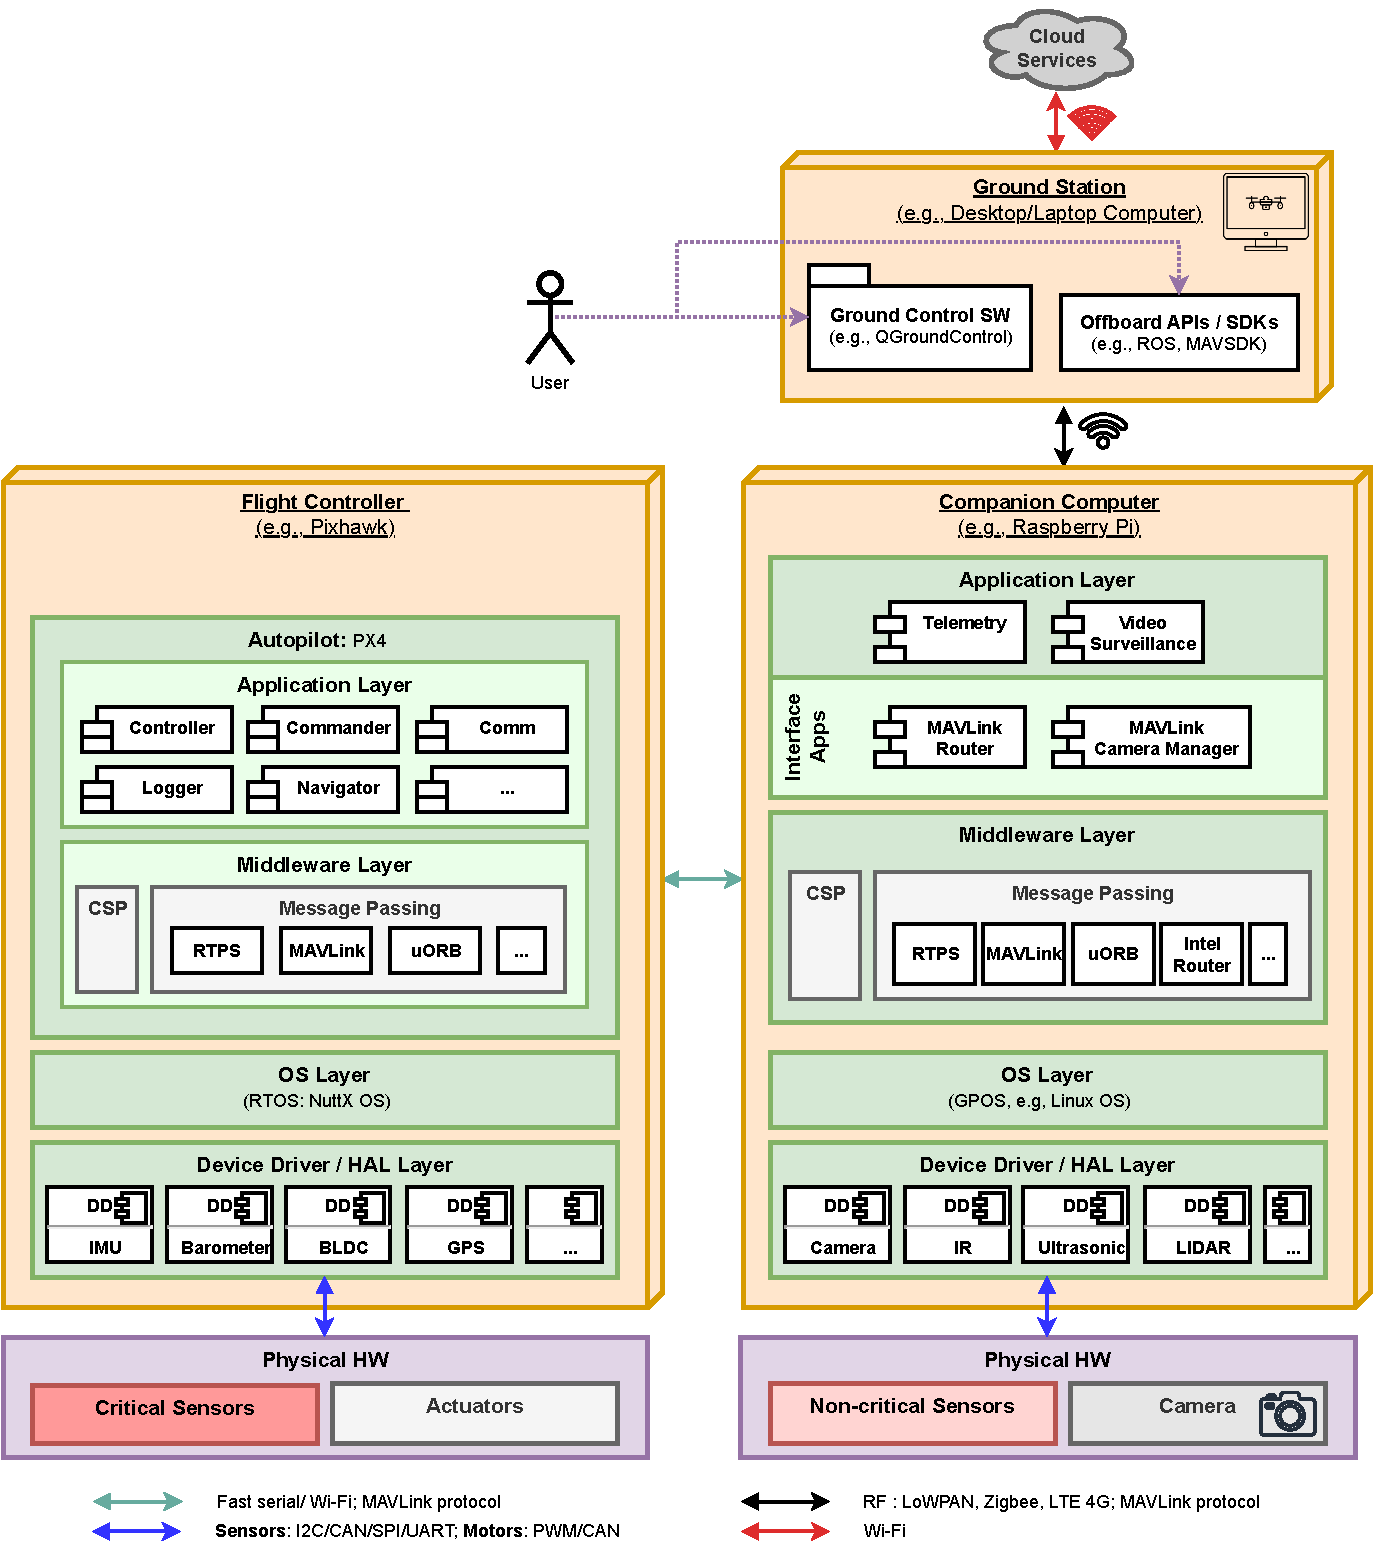
\includegraphics[width=0.9\textwidth]{./img/pdf/uav-main-design-conv-sol-1.pdf} 
%  \includesvg[width=1.0\textwidth]{./img/virtualization.svg} 
  %\caption[Virtualization mind map]{Virtualization mind map}%
  \caption{UAV design: conventional solution --- full}%
  \label{fig:uav-design-conv-sol-1}
\end{figure}

The PX4 flight controller stack was selected for this work due to its
open-source nature, extensive platform support, modular architecture, and
widespread adoption in the industry. PX4 runs on the flight controller on top of
the NuttX \gls{rtos}. In the generic case, the companion computer is used to
route communications between the \gls{gcs} and the \gls{fmu}: a fast serial
link, typically \gls{uart} or Ethernet, is established between the \gls{fmu} and
the companion computer using the MAVLink protocol; the companion computer
runs extra software to route the MAVLink traffic,
e.g. MAVLink Router~\cite{px4-routers}.
%
The \lstinline{User} interacts with the \gls{gcs} software, specifically
\lstinline{QGroundControl}, selected for its open-source model and compatibility
with the PX4 flight stack. The \lstinline{User} can also interact with the
Companion Computer via offboard \glspl{api} and \glspl{sdk} (e.g.,
\lstinline{MAVSDK}). The \gls{rc} link is omitted, as it is only useful in
manual mode and therefore not relevant to the video-surveillance application.

In the vast majority of cases, extra software, running on the companion
computer, is required to interface the camera, e.g. the Mavlink Camera Manager~\cite{px4-cam-managers}. This
component acts as bridge between the \gls{fmu} and \gls{gcs} and a translator between the MAVLink Camera Protocol v2
(used by PX4) and the native protocol of the camera~\cite{px4-cam-managers}.
%
This communication routing poses an increased risk to the \gls{uav}: if the
companion computer is compromised the \gls{fmu} may malfunction due to data
corruption or communication loss. Furthermore, the additional software required
to route MAVLink traffic and manage the camera adds complexity and latency to
the system.

Fig.~\ref{fig:uav-design-conv-sol-2} showcases a simplified conventional
solution customized for video surveillance, with a higher degree of
decoupling.

\begin{figure}[!hbt]
  \centering
  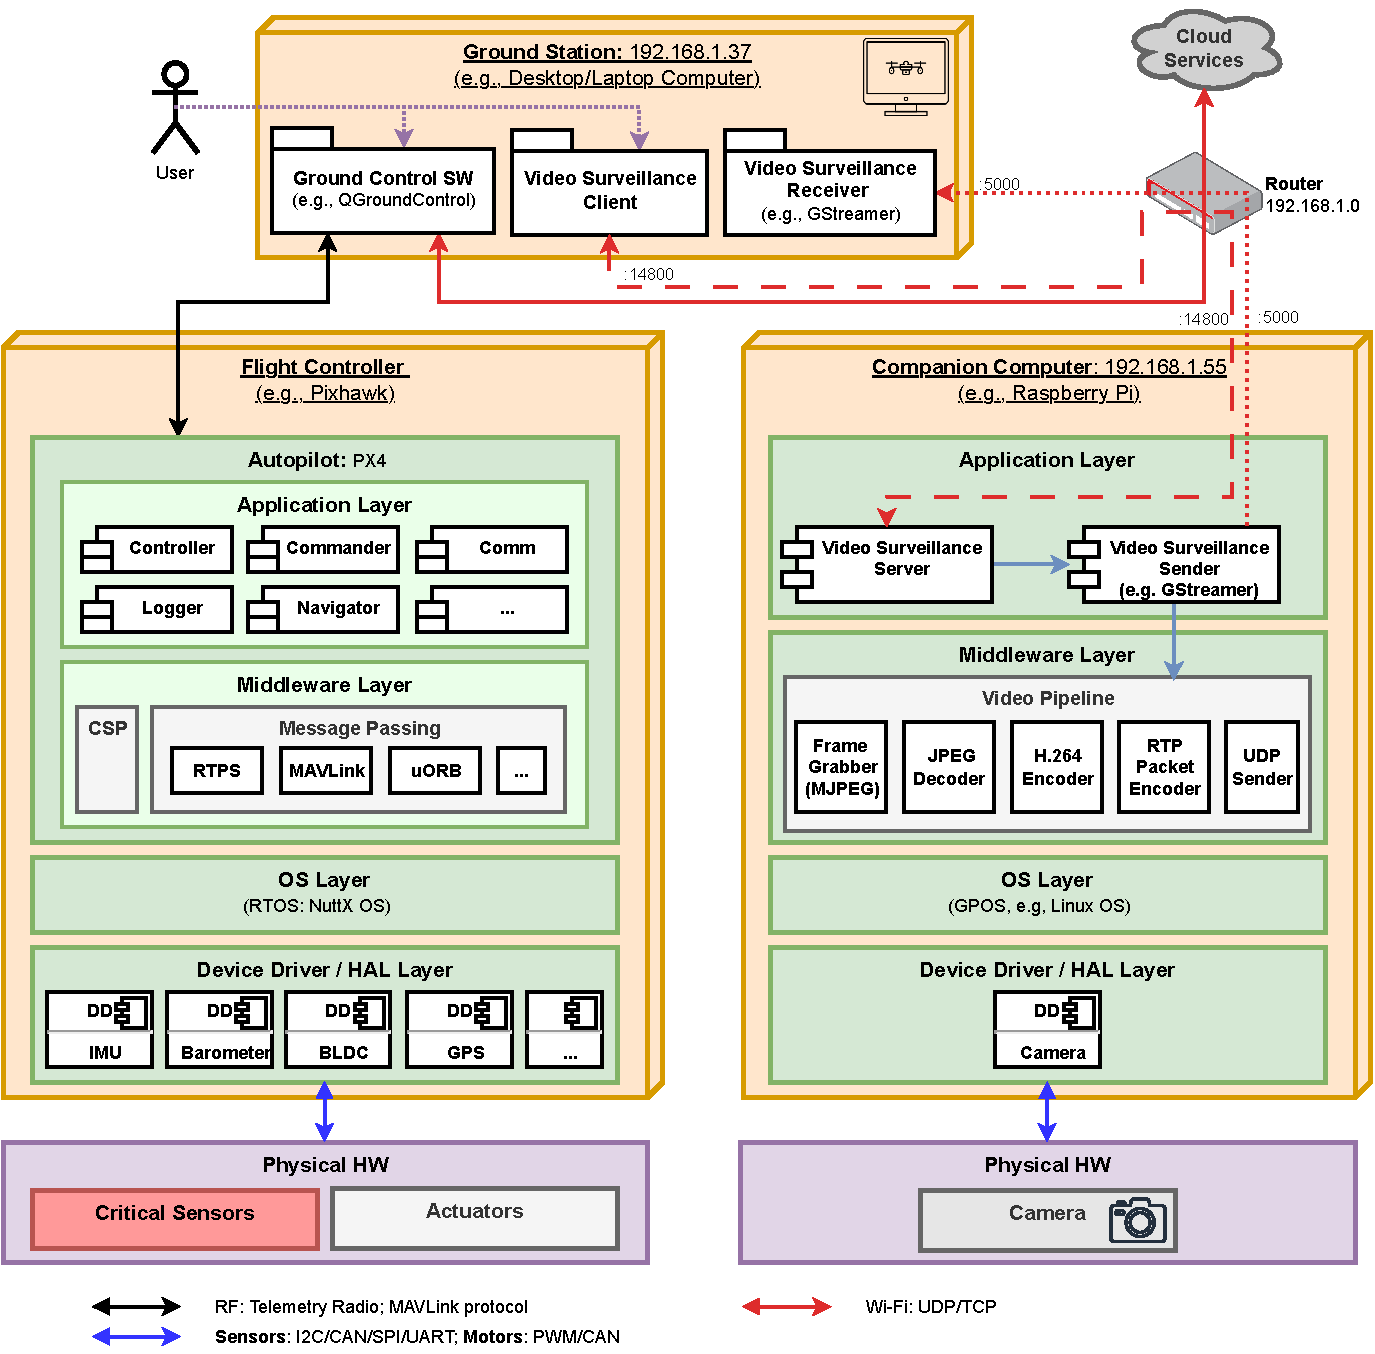
\includegraphics[width=0.9\textwidth]{./img/pdf/uav-main-design-conv-sol-2.pdf} 
  \caption{UAV design: conventional solution --- simplified}%
  \label{fig:uav-design-conv-sol-2}
\end{figure}

Dedicated
communication links are established for communication between the \gls{gcs} and \gls{fmu} (telemetry radio) and the
camera (Wi-Fi). To streamline the network configuration and eliminate the need
for additional hardware, the \gls{gcs} and the \gls{uav} are integrated into the
same \gls{lan}. The video surveillance software is also simplified consisting of
a client running on the \gls{gcs} and the server running on the companion
computer supported by a suitable video pipeline and device drivers. The
client runs on port 5000 of the \gls{gcs} issuing command for the server running
on the same port in the Companion Computer. The server handles commands and
requests the sender to setup the video pipeline and transmit video frames back
to the \gls{gcs}. The receiver sets up a video pipeline on the \gls{gcs} (not
displayed) that processes the video frames and displays it to the \lstinline{User}.

On the receiving end of the video surveillance system (\gls{gcs}), occasional
frame loss is tolerable and does not compromise situational awareness of the
target area. Consequently, a communication protocol without delivery guarantees,
such as \gls{udp}, is appropriate.
%
This simplified conventional solution forms the base design for the platform
unification.

\subsection{Unsupervised Single-Platform Flight Stack}
\label{sec:unsuperv-stack}
Integration of the \gls{fmu} and companion computer platforms requires
encapsulation of their functionalities into standalone components within a
unified platform. In the \glsxtrfull{uspfs}, these components are abstracted as
processes running on a \gls{gpos}.
%
Fig.~\ref{fig:uav-design-unsup} illustrates the \gls{uspfs} system
architecture. Software processes for the \gls{gcs} and \gls{uavic} appear in
blue. The \gls{uavic} consolidates both \gls{fmu} and companion computer nodes
onto a single platform operating on a \gls{gpos} (specifically Linux), with PX4
executing on core 0 and remaining cores allocated to the video surveillance
application.

\begin{figure}[!hbt]
  \centering
  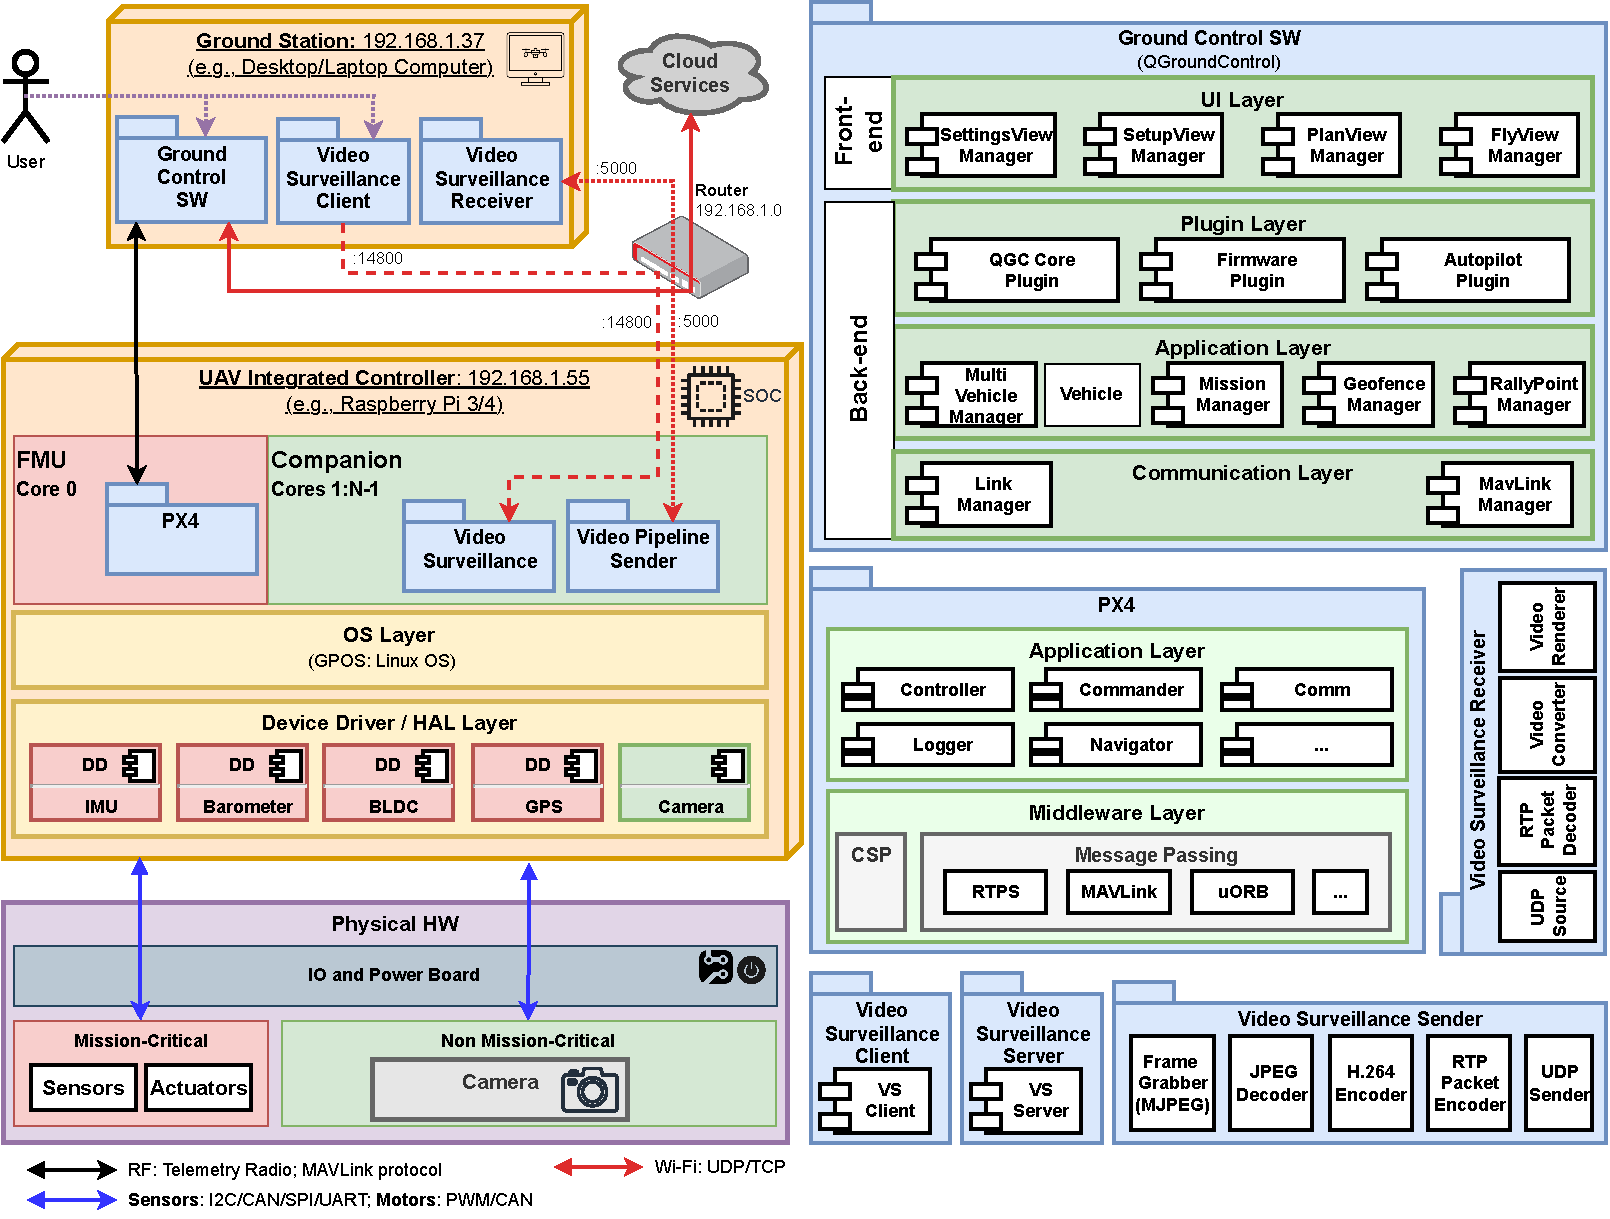
\includegraphics[width=1.0\textwidth]{./img/pdf/uav-main-design-unsup.pdf} 
%  \includesvg[width=1.0\textwidth]{./img/virtualization.svg} 
  %\caption[Virtualization mind map]{Virtualization mind map}%
  \caption{UAV design: Unsupervised Single-Platform Flight Stack}%
  \label{fig:uav-design-unsup}
\end{figure}

It is important to note that PX4 no longer runs on the Nuttx \gls{rtos}, which
may introduce challenges in meeting the soft real-time requirements of the flight
control. To address this, one core is explicitly dedicated to the PX4
application. Additionally, employing a real-time Linux kernel with a suitable
\gls{io} scheduler can help mitigate timing issues.
%
However, this architecture lacks isolation between systems, meaning a failure in
the non-critical system can propagate to the \gls{fmu}. Such failures could lead
to \gls{fmu} malfunctions, potentially resulting in a crash with unpredictable
consequences. As mentioned earlier, this solution alone is insufficient;
supervision is essential to ensure both reliable consolidation and safe
integration.

\subsection{Supervised Single-Platform Flight Stack}
\label{sec:superv-stack}
Fig.~\ref{fig:uav-design-sup} illustrates the system architecture of the
\glsxtrfull{sspfs}. In this design, the functionalities of the \gls{fmu} and
companion computer are abstracted as guest \glspl{vm} running atop the Bao
Hypervisor in the \gls{uavic} node. This approach ensures isolation between the two mixed-criticality
systems, preventing faults in the non-critical system from impacting the
\gls{fmu} and causing potential malfunctions.

\begin{figure}[!hbt]
  \centering
  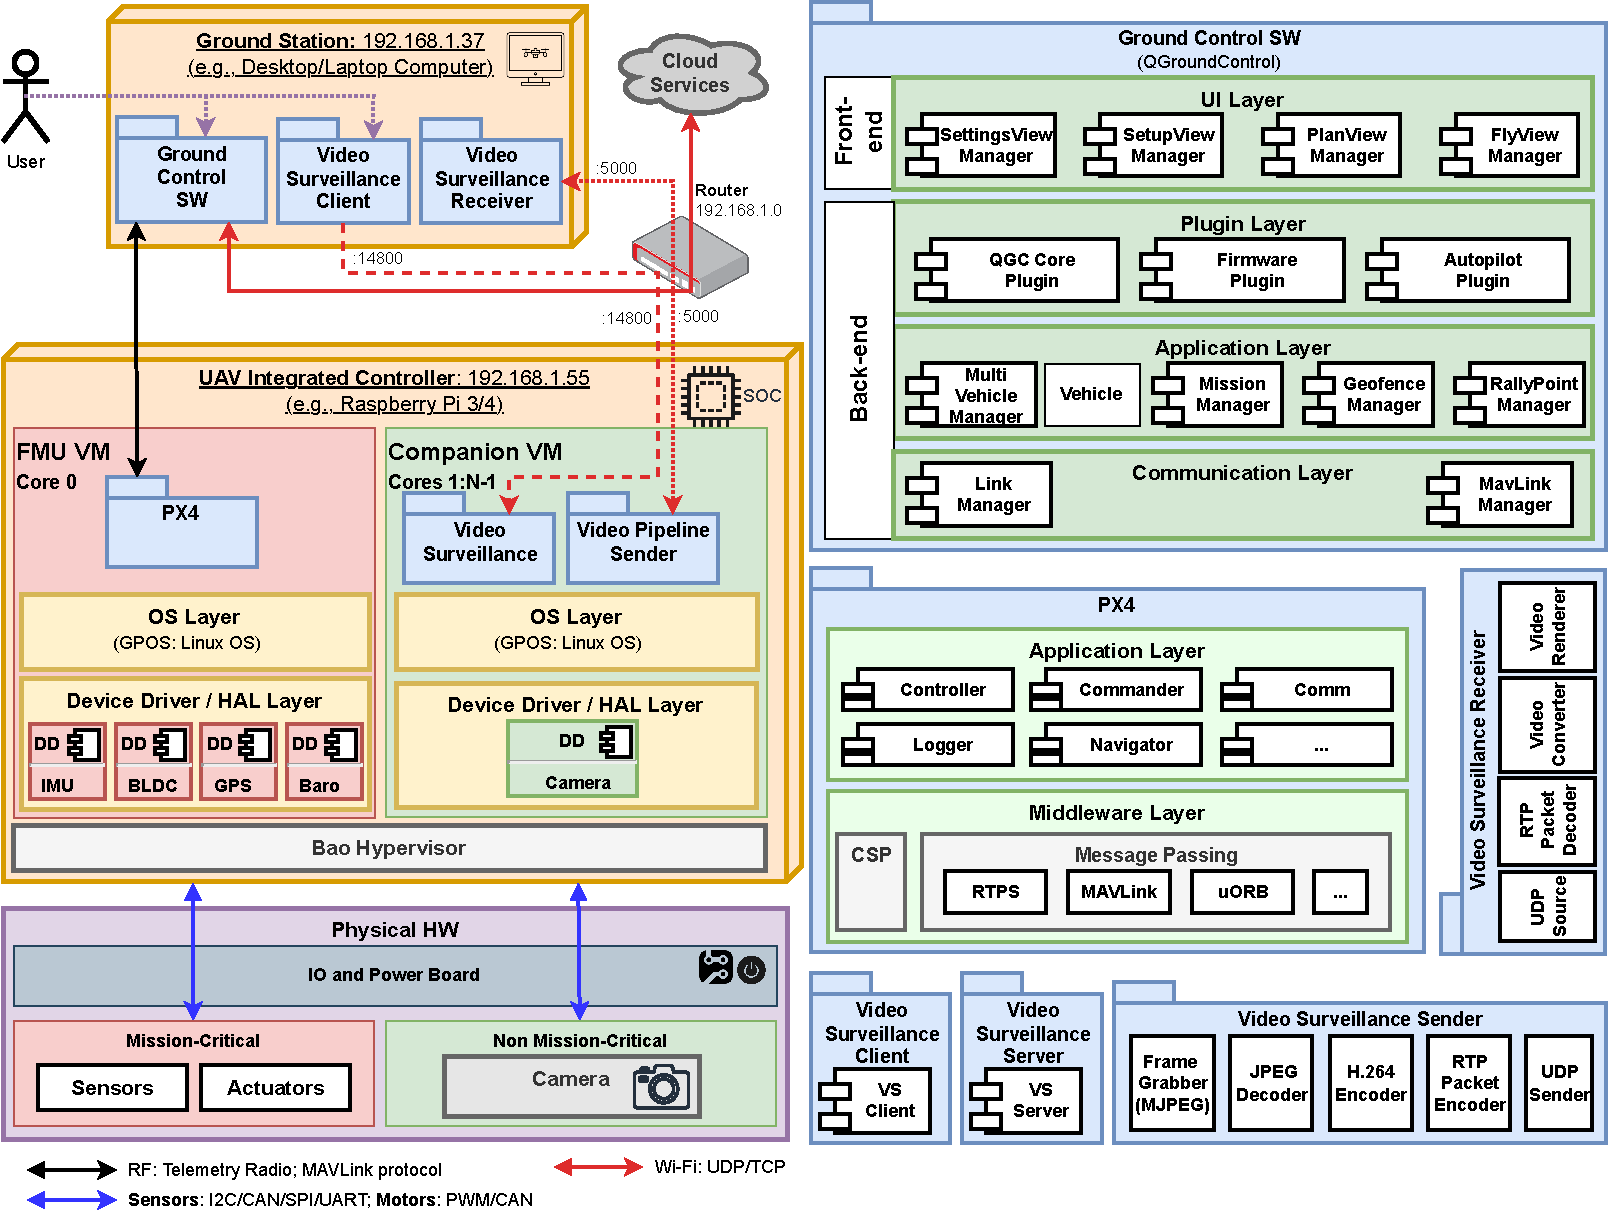
\includegraphics[width=1.0\textwidth]{./img/pdf/uav-main-design-sup.pdf} 
%  \includesvg[width=1.0\textwidth]{./img/virtualization.svg} 
  %\caption[Virtualization mind map]{Virtualization mind map}%
  \caption{UAV design: Supervised Single-Platform Flight Stack}%
  \label{fig:uav-design-sup}
\end{figure}

Each \gls{vm} operates a Linux-based \gls{os}, enabling further
customization. For instance, the \gls{fmu} \gls{vm} can utilize a real-time
kernel, providing additional guarantees that its assigned core remains fully
dedicated to its execution. Meanwhile, the Companion \gls{vm} can operate with a
standard Linux kernel. Bao's static partitioning mechanism guarantees that the
hardware resources assigned to each \gls{vm} are strictly dedicated, ensuring
isolation. Moreover, device drivers within each \gls{vm} are specific to that
\gls{vm}, minimizing the impact of software bugs or failures.

However, this approach requires each \gls{vm} to include a full \gls{os},
leading to larger binary sizes. Additionally, the \lstinline{User} must carefully
select and allocate hardware resources to avoid conflicts between \glspl{vm}
while maintaining adequate performance in terms of \gls{ram}, available
\glspl{cpu}, and other critical resources. This requires a deeper knowledge
about the hardware used. As such, the system architecture may require later
adaptation to the selected hardware.

\section{Hardware Selection}
\label{sec:hardware-selection}
In this section, the hardware for the \gls{uav}, \gls{uavic}, and
extra addons are selected. The hardware is mapped to comply with PX4
requirements and the \gls{uavic} restrictions imposed by Bao.

\subsection{UAV}
\label{sec:uav-hw-sel}
We begin by defining the \gls{uav}'s target characteristics. A multirotor
airframe is preferable because it is low-cost, widely available, compact, and
provides \gls{vtol} capability to reduce takeoff area.
Additionally, the
\gls{uav} must fly in low altitudes due to regulatory and operational
constraints. We must also optimize the \gls{uav}'s power/weight ration to extend
flight auto.
%
Fig.~\ref{fig:hoverGames-drone} shows the selected \gls{uav}, the
\lstinline{KIT-HGDRONEK66}, commonly referred to as the NXP HoverGames \gls{uav}
kit~\cite{nxp-hoverGames-uav}. This \gls{diy} professional development kit,
priced under 500 USD, features the RDDRONE-FMUK66 as the \gls{fmu} unit (1).

\begin{figure}[!hbt]
  \centering
  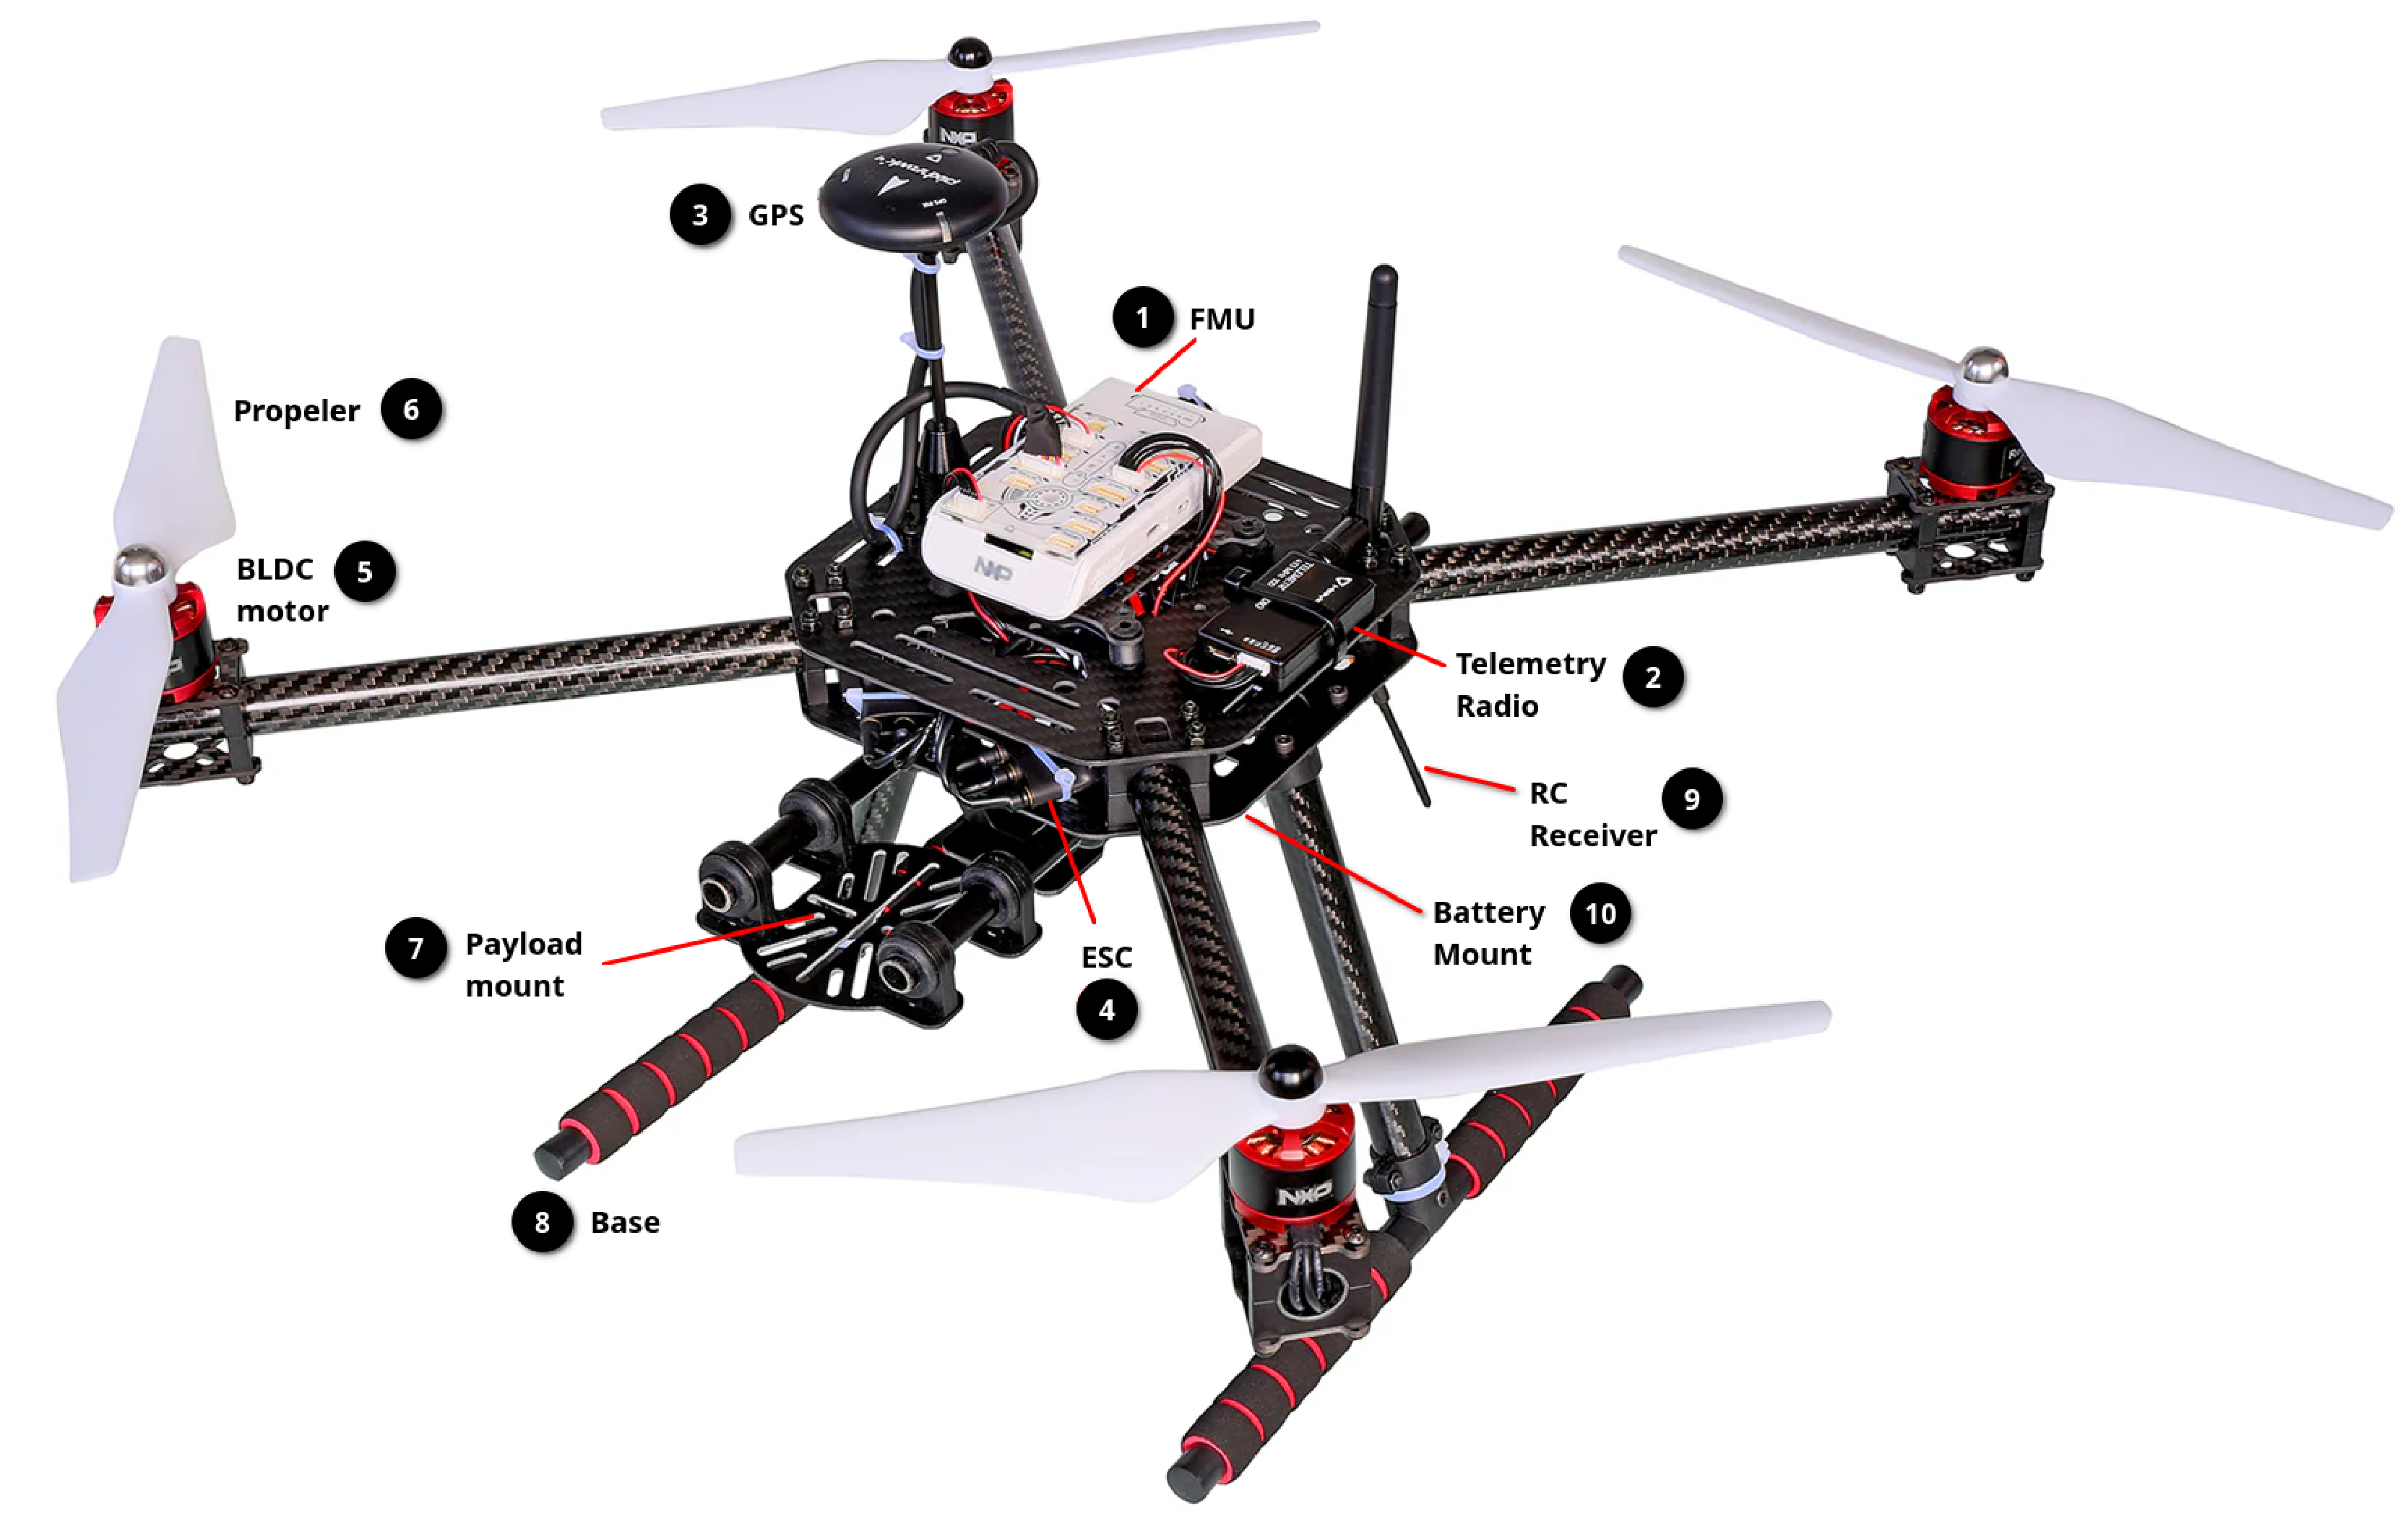
\includegraphics[width=1.0\textwidth]{./img/pdf/hoverGames-drone.pdf} 
  \caption[NXP HoverGames UAV kit]{NXP HoverGames UAV kit (adapted from~\cite{nxp-hoverGames-uav})\footnotemark}%
  \label{fig:hoverGames-drone}
\end{figure}
%
\fnlicNC{NXP Semiconductors}

The kit is built on an S500 carbon fiber frame with four rotors (quadcopter) and
has a 500-millimeter wheelbase (diagonal distance between opposing motors). It
employs \gls{bldc} motors (5) to drive the propellers (4), which are controlled
by individual \gls{esc} units (4).
%
For autonomous flight capabilities, the kit includes a \gls{gps} module (3) and a payload mount (7) designed for accessories such as cameras. Power is supplied via a 3S \gls{lipo} battery (sold separately) with a capacity ranging from 3500 to 5000 mAh.
%
Additionally, a telemetry radio (2), also sold separately, can be connected to
the \gls{fmu} (1). This telemetry module operates in the 433 MHz frequency band
in Europe, enabling remote communication and monitoring.
%
The kit also includes the \gls{rc} remote
controller GS-i6S transmitter and receiver modules.

Fig.~\ref{fig:hoverGames-blkDiag} depicts the block diagram for the NXP
HoverGames \gls{uav} kit.  It features the RDDRONE-FMUK66 \gls{fmu}, which uses 
Kinetis\textreg K66 \gls{mcu} (180 MHz, 2 MB of flash and 256 KB of \gls{sram}), based on
the 32-bit Arm\textreg Cortex\textreg--M4 Core)~\cite{nxp-hoverGames-fmu},
running the PX4 autopilot stack.
%
The kit includes a power module and a power-distribution board with current and
voltage sensing to estimate \gls{lipo} battery autonomy. The power-distribution
board supplies the \gls{bldc} motors, which are driven by the \gls{esc} via
\gls{pwm}. A SEGGER J-Link EDU Mini \gls{swd} adapter supports on-target
debugging and firmware upload to the \gls{fmu}.
%
Common \gls{uav} sensors are supported, including an accelerometer, gyroscope,
magnetometer (compass), and barometer. The \gls{fmu} communicates with the
companion computer over \gls{uart}, and with the \gls{gcs} via a telemetry radio
or an \gls{rc} link. An optional \gls{sd} card enables flight logging for
offline analysis, debugging, and replay in simulation tools.

\begin{figure}[!hbt]
  \centering
  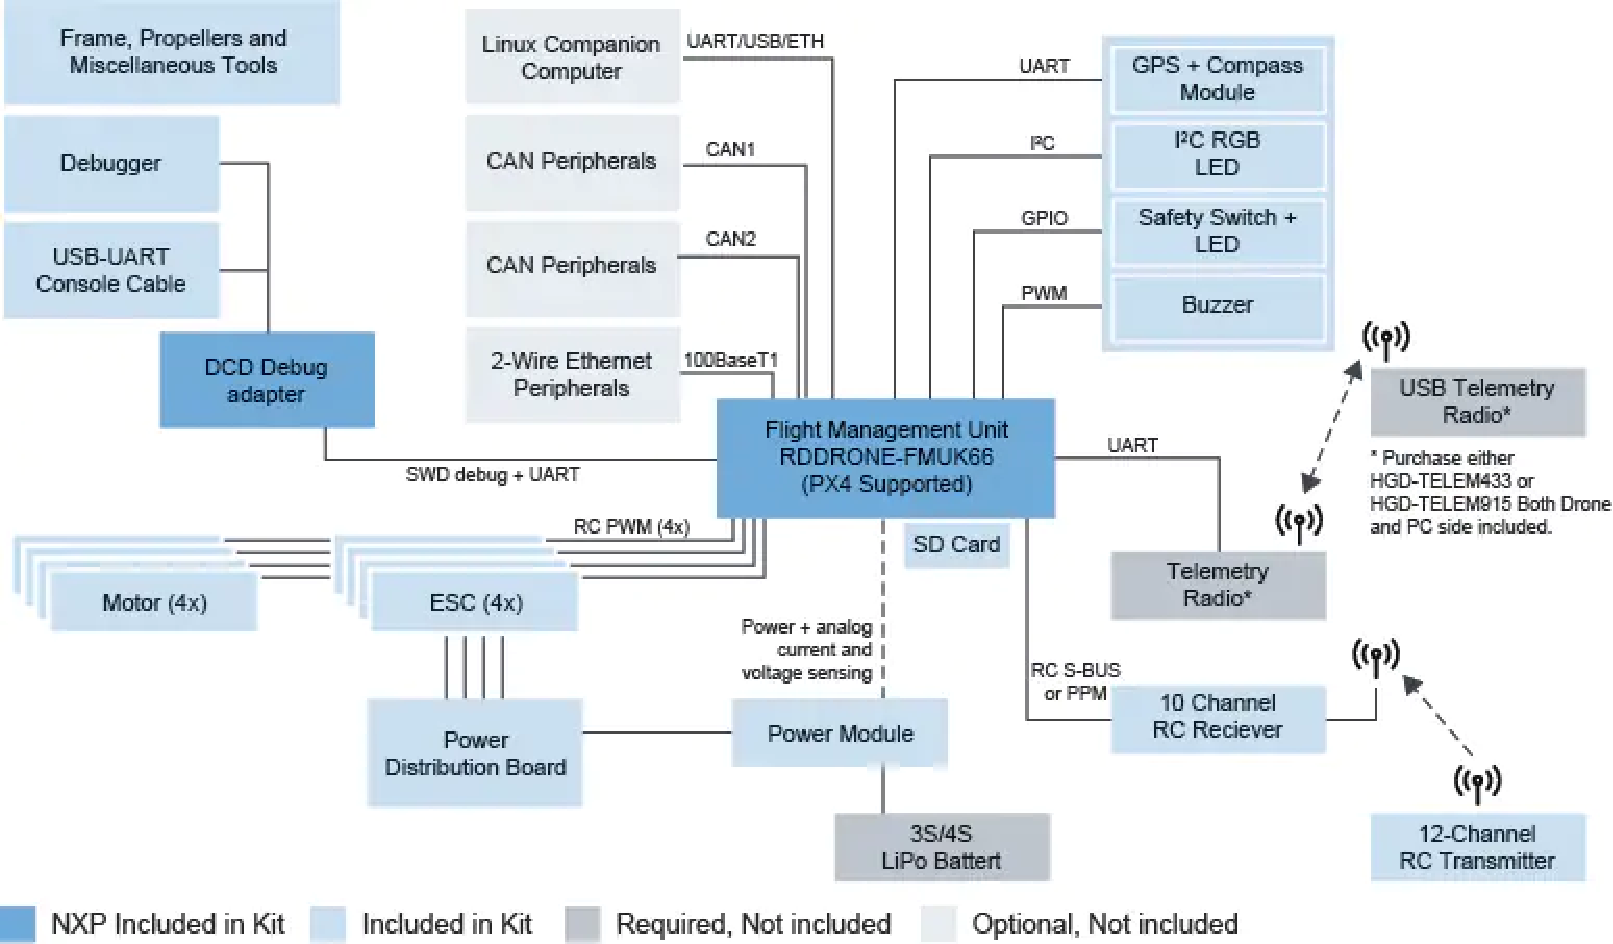
\includegraphics[width=1.0\textwidth]{./img/pdf/hoverGames-blkDiag.pdf} 
  \caption[NXP HoverGames block diagram]{NXP HoverGames block diagram (withdrawn from~\cite{nxp-hoverGames-uav})\footnotemark}%
  \label{fig:hoverGames-blkDiag}
\end{figure}
%
\fnlicNC{NXP Semiconductors}


\subsection{UAV Integrated Controller}
\label{sec:uav-integr-contr}
The \glsxtrfull{uavic} merges \gls{fmu} and companion-computer functionality on
a single platform. For mixed-criticality, the ideal design separates computing
domains: e.g., a real-time processor for the \gls{fmu} and a general-purpose
processor for the companion stack. This points to a heterogeneous \gls{soc},
such as the NXP i.MX~8M Nano~\cite{imx8mn}, which integrates an Arm Cortex-M7
(well suited to NuttX) and a quad-core Arm Cortex-A53 (well suited to a Linux
\gls{os}). However, the NuttX \gls{rtos} does not currently support this board~\cite{nuttx-platforms}.

Our initial plan was to port NuttX to the Cortex-M7 and then port PX4 to that
NuttX target, including all required device drivers. In parallel, we would also
need Bao support for this board. The combined effort -- new NuttX port, PX4
enablement, and Bao enablement -- proved impractical for this work's scope, so
we pivoted to a more direct path.
%
We next considered running PX4 directly on Linux with a real-time kernel and
appropriate \gls{io} scheduling to limit latency. PX4’s Linux support, however,
is restricted to a small set of platforms (e.g., BeagleBone Blue and
Raspberry~Pi~2/3/4 with specific shields)~\cite{px4-experimental-autopilot},
which constrained our options.
%
Consequently, we consolidated each software stack into its own Linux \gls{os}
\gls{vm}, rather than splitting across heterogeneous cores.

As the host
platform, we selected Raspberry~Pi~4 paired with the PilotPi shield, balancing
availability, documentation quality, and cost. Fig.~\ref{fig:pilotpi-annot}
shows the resulting \gls{uavic}.
%
The Raspberry Pi 4 Model B (1) operates a Linux-based \gls{os}
from the \gls{sd} card, directly exposing the \gls{csi} camera and
\gls{usb} interfaces. This model features the Broadcom BCM2711
\gls{soc}, containing a 64-bit quad-core Arm\textreg Cortex\textreg--A72 \gls{cpu} at
1.8 GHz and VideoCore VI \gls{gpu} at 500 MHz~\cite{rpi4-specs,rpi4-bcm2711},
with 8 GB LPDDR4-3200 SDRAM. Connectivity includes dual-band 802.11ac wireless,
Bluetooth 5.0, Gigabit Ethernet, two \gls{usb} 3.0 ports, and two \gls{usb} 2.0 ports.
%
The sensor board (2) mounts atop the Raspberry Pi,
providing \gls{gps}, telemetry, and \gls{rc} external interfaces mapped to
\lstinline{/dev/ttySC0}, \lstinline{/dev/ttySC1}, and \lstinline{/dev/ttyAMA0},
respectively. Onboard sensors include an accelerometer/gyroscope
(\lstinline{ICM42688P}), magnetometer (\lstinline{IST8310}), and barometer
(\lstinline{MS5611}) required by PX4.
%
The topmost layer contains the power board (3), handling power supply (8),
monitoring (11), and motor actuation via \gls{pwm} (10) supported by the Linux
\lstinline{PCA9685} driver. A header exposes unused pins, enabling additional
connections such as a remote serial interface (UART5).

\begin{figure}[!hbt]
  \centering
  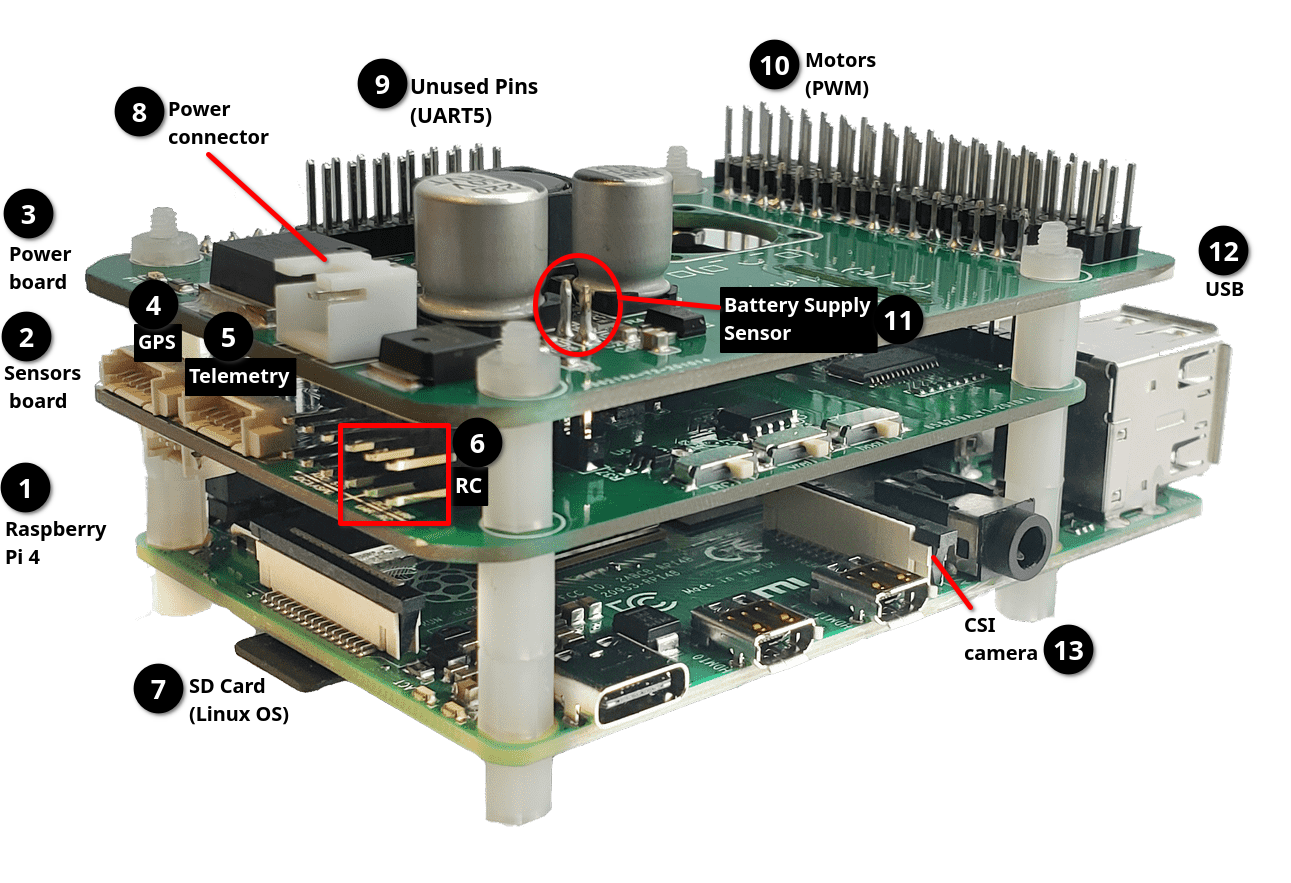
\includegraphics[width=0.9\textwidth]{./img/png/pilotpi-annotated} 
  \caption[UAVIC: Raspberry Pi 4 + PilotPi shield]{UAVIC: Raspberry Pi 4 +
    PilotPi shield (adapted from~\cite{px4-pilotpi})\footnotemark}%
  \label{fig:pilotpi-annot}
\end{figure}
%
%\fnlicReq{Elsevier}{5457890117132}%
\fnlicCCFour{foot:pilotpi-annotated}%



% Fig.~\ref{fig:pilotpi-annot} presents the selected \gls{uavic}: the Raspberry Pi
% 4 with PilotPi shield. This combination was chosen for its detailed documentation
% and cost efficiency.

% The PilotPi shield provides a fully functional open-source
% solution for running PX4 autopilot directly on Raspberry Pi, requiring no
% proprietary drivers while offering open-source \gls{pcb} and
% schematics~\cite{px4-pilotpi}.

% \begin{figure}[!hbt]
%   \centering
%   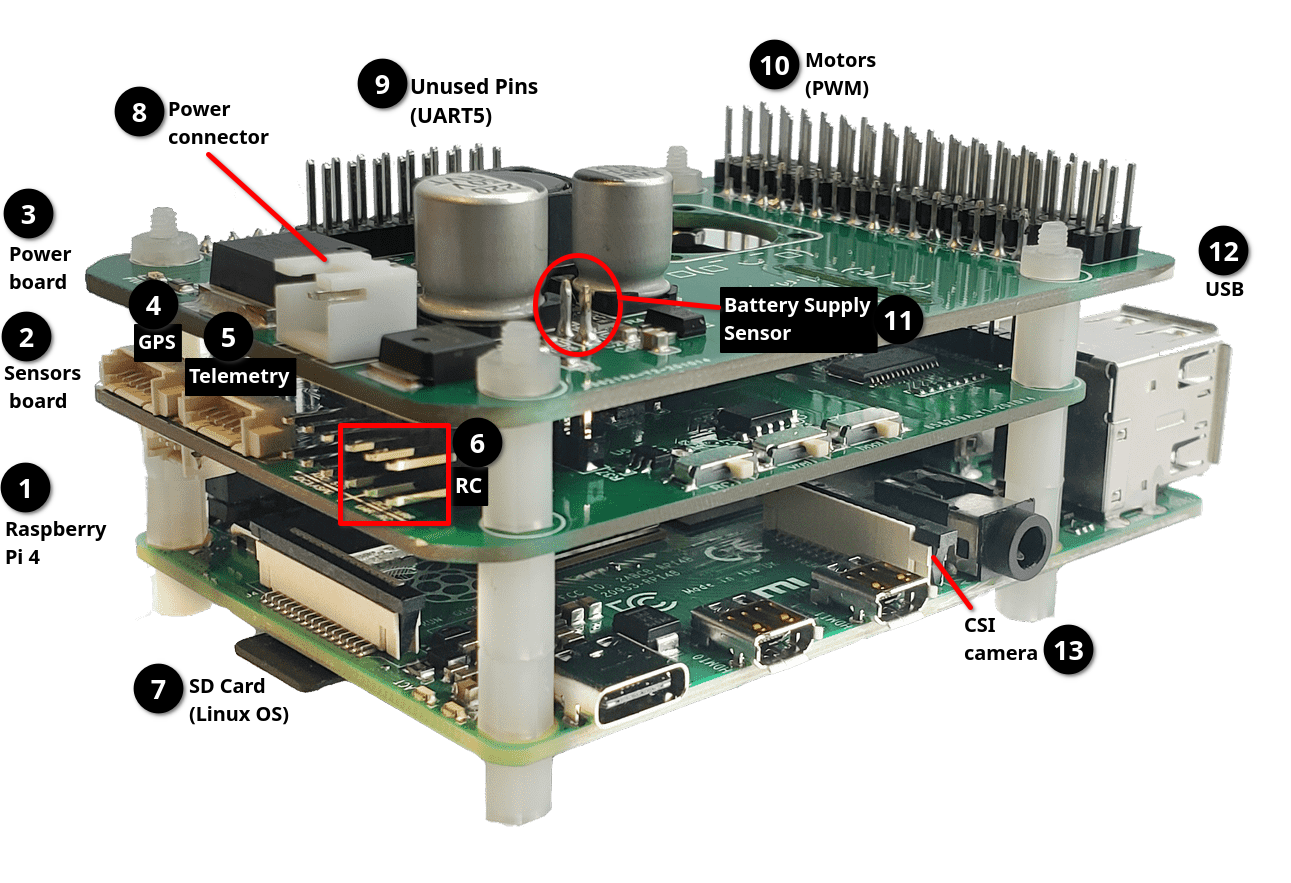
\includegraphics[width=1.0\textwidth]{./img/png/pilotpi-annotated} 
%   \caption[UAVIC: Raspberry Pi 4 + PilotPi shield]{UAVIC: Raspberry Pi 4 +
%     PilotPi shield (adapted from~\cite{px4-pilotpi})\footnotemark}%
%   \label{fig:pilotpi-annot}
% \end{figure}
% %
% %\fnlicReq{Elsevier}{5457890117132}%
% \fnlicCCFour{foot:pilotpi-annotated}%

% The Raspberry Pi 4 Model B (1) operates a Linux-based \gls{os}
% from the \gls{sd} card, directly exposing the \gls{csi} camera and
% \gls{usb} interfaces. This model features the Broadcom BCM2711
% \gls{soc}, containing a 64-bit quad-core Arm\textreg Cortex\textreg--A72 \gls{cpu} at
% 1.8 GHz and VideoCore VI \gls{gpu} at 500 MHz~\cite{rpi4-specs,rpi4-bcm2711},
% with 8 GB LPDDR4-3200 SDRAM. Connectivity includes dual-band 802.11ac wireless,
% Bluetooth 5.0, Gigabit Ethernet, two \gls{usb} 3.0 ports, and two \gls{usb} 2.0 ports.

% The sensor board (2) mounts atop the Raspberry Pi,
% providing \gls{gps}, telemetry, and \gls{rc} external interfaces mapped to
% \lstinline{/dev/ttySC0}, \lstinline{/dev/ttySC1}, and \lstinline{/dev/ttyAMA0},
% respectively. Onboard sensors include an accelerometer/gyroscope
% (\lstinline{ICM42688P}), magnetometer (\lstinline{IST8310}), and barometer
% (\lstinline{MS5611}) required by PX4.

% The topmost layer contains the power board (3), handling power supply (8),
% monitoring (11), and motor actuation via \gls{pwm} (10) supported by the Linux
% \lstinline{PCA9685} driver. A header exposes unused pins, enabling additional
% connections such as a remote serial interface (UART5).

\subsection{Hardware mapping}
\label{sec:hardware-mapping}
The \gls{uavic} platform must satisfy PX4 requirements for sensors and
actuators. Because the Bao hypervisor enforces static partitioning, we must also
determine whether the \gls{uavic} hardware can be made fully available to each
guest in the \gls{sspfs} solution or if alternatives are needed.
Accordingly, we first map the PX4-required hardware to the Linux device tree for
the \gls{uspfs} solution and then adapt that mapping to meet Bao’s constraints in the \gls{sspfs} implementation.

\subsubsection{USPFS}
\label{sec:base-scenario}
Fig.~\ref{fig:hw-map-1} depicts the full device tree for the \gls{uavic} system,
representing the \gls{uspfs} solution (base scenario).
The solid lines represent aggregation, e.g., the \lstinline{root} node includes the \lstinline{memory} node. The
dashed lines represent dependency, e.g., the \lstinline{power} and \lstinline{firmware} nodes depend on the \lstinline{mailbox}.
%
The device tree coloring scheme highlights functional groupings:
% \begin{itemize}[noitemsep,topsep=0pt]
\begin{itemize}
%
\item \hlighthex{ADD8E6}{000000}{Generic nodes}: essential for all Raspberry Pi
  4 configurations: \lstinline{memory}, \lstinline{cpu},
  \lstinline{power-regulator}, etc.
%
\item \hlighthex{FFE4C4}{000000}{PX4-required nodes}: \lstinline{i2c1} (motor
  actuation), \lstinline{spi0} (\gls{imu}; barometer; magnetometer),
  \lstinline{spi1} (\gls{gps}; telemetry radio), and \glspl{uart} 0/5 (\gls{rc}
  link; debug console)
%
\item \hlighthex{90EE90}{000000}{Companion VM nodes}: \lstinline{i2c0} and
  \lstinline{csi1} (camera interface), \lstinline{mmcnr} (Wi-Fi support)
%
\item \hlighthex{FFB6C1}{000000}{Firmware nodes}: Enable \gls{gpu}-\gls{cpu} communication via \lstinline{mailbox}~\cite{rpi4-fw-mbox}
\end{itemize}

\begin{figure}[!hbt]
  \centering
  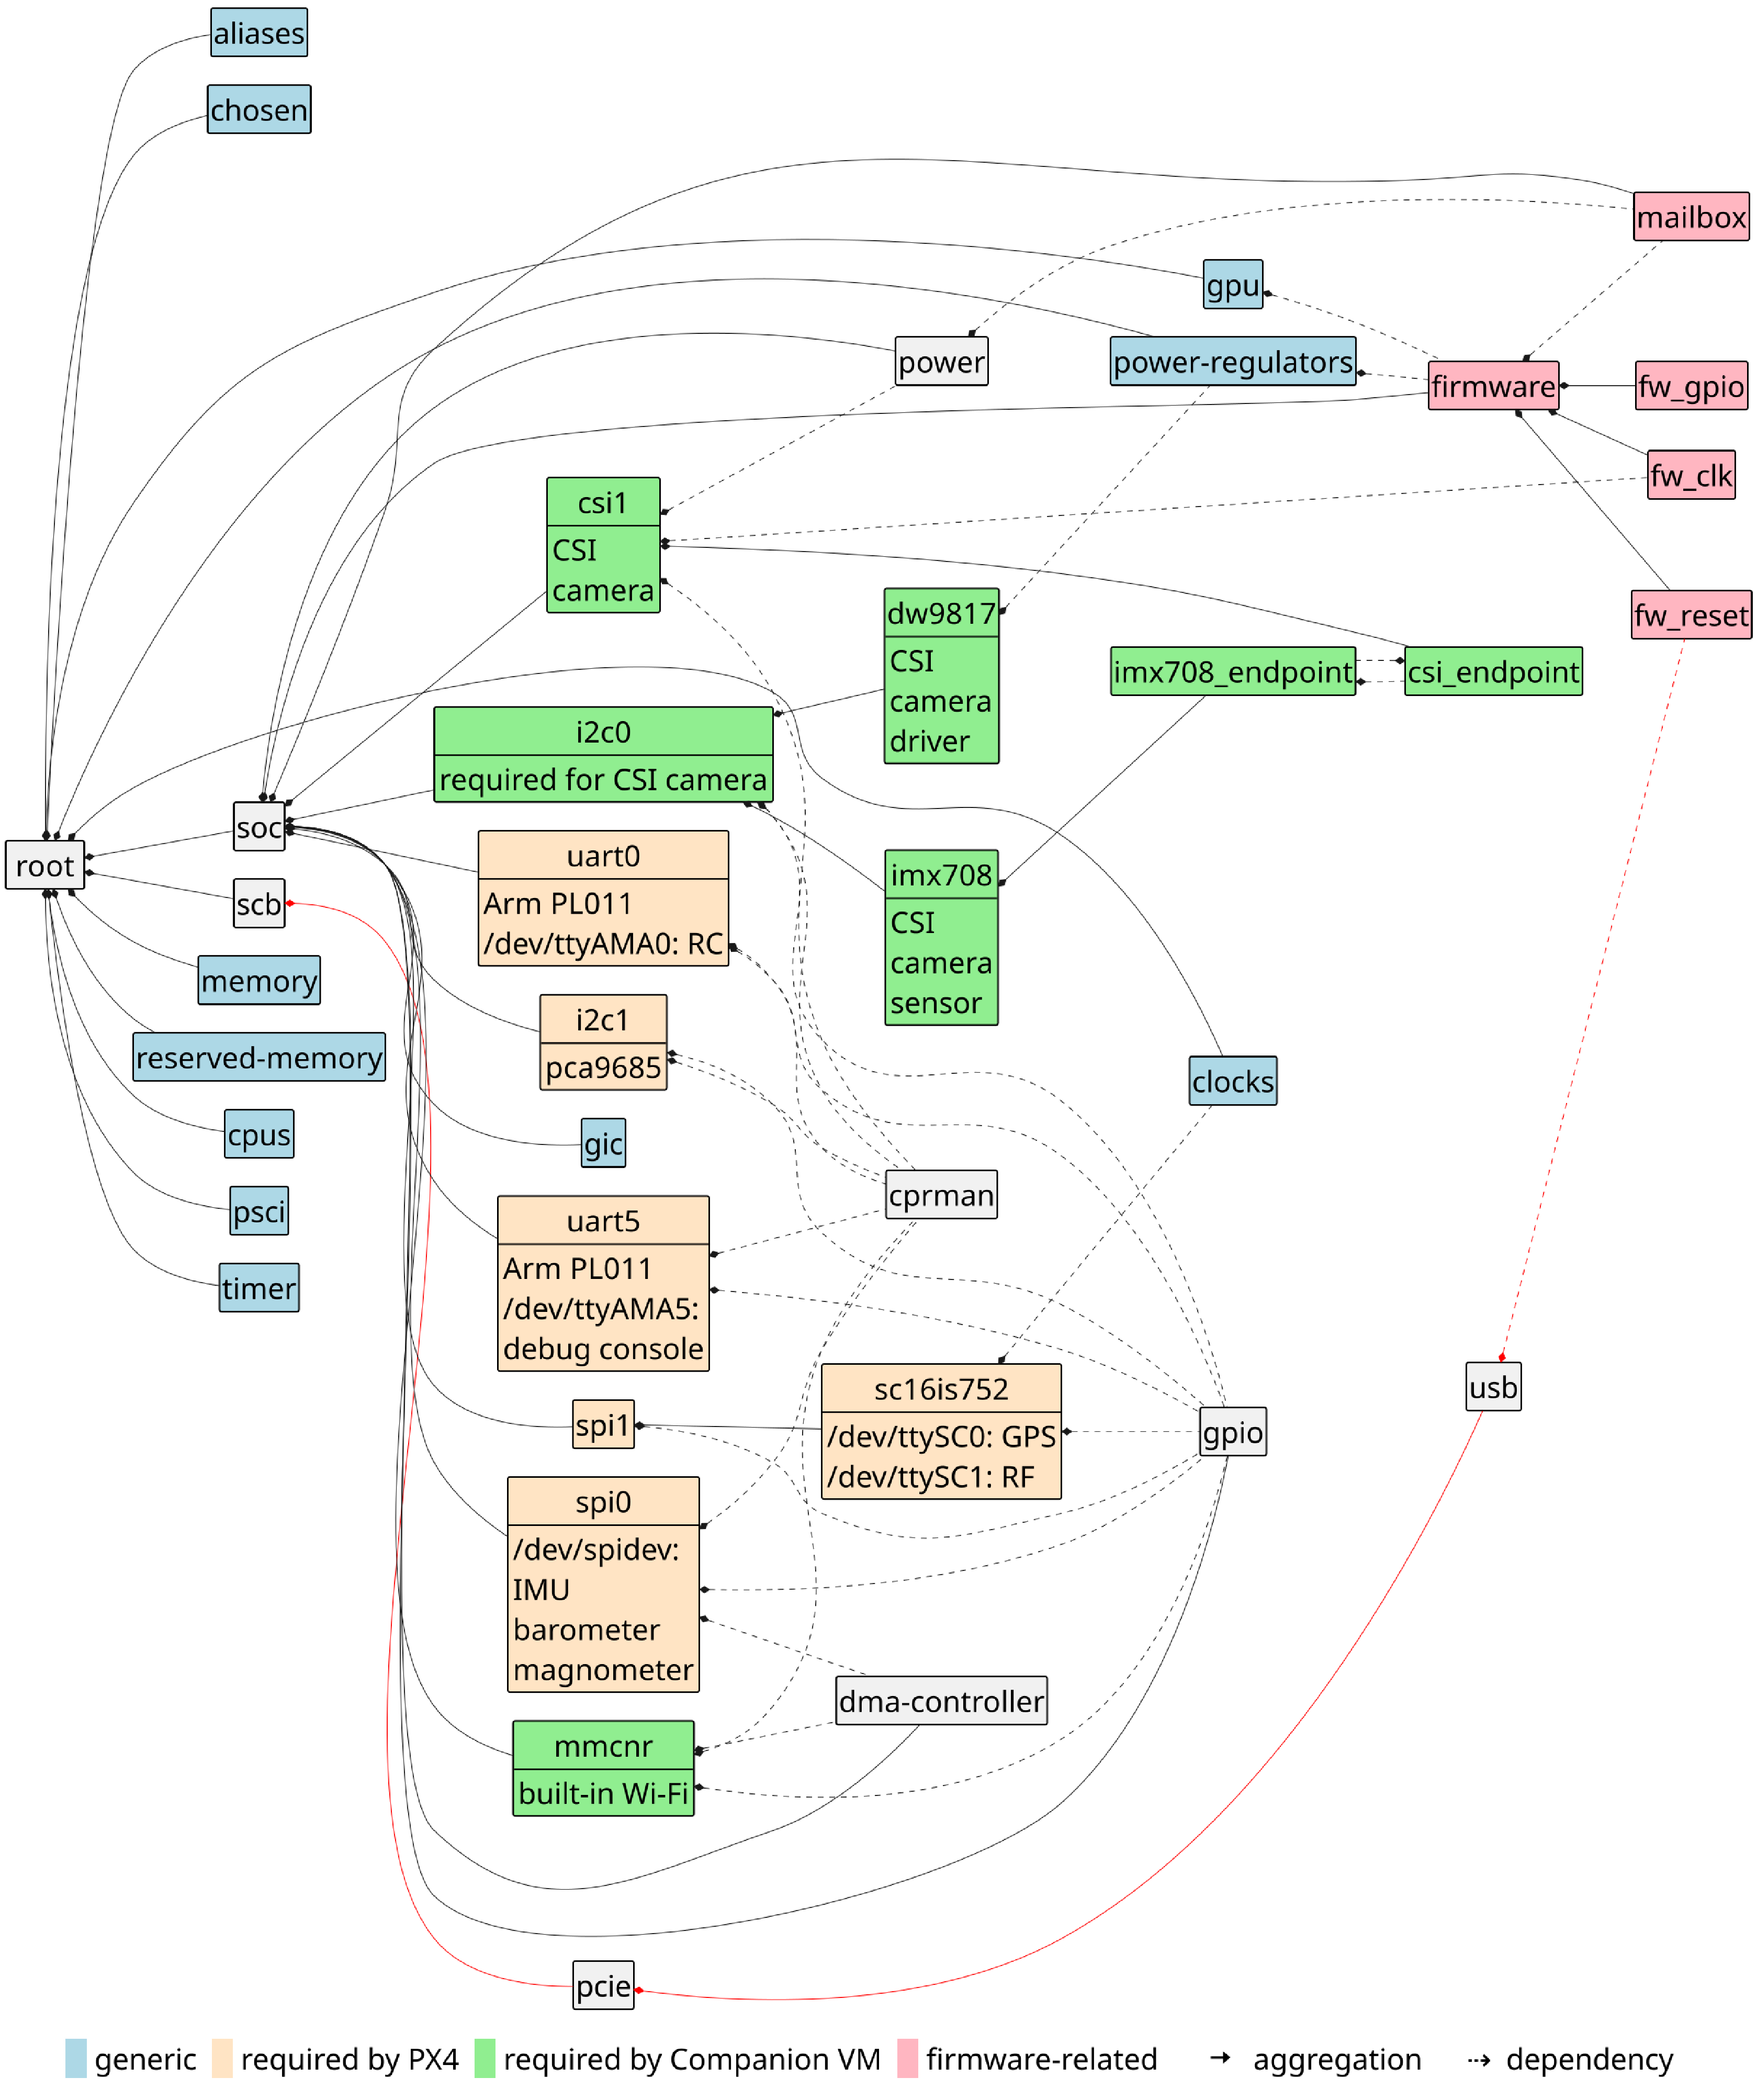
\includegraphics[width=0.85\textwidth]{./img/pdf/hw-map-1} 
  \caption[Hardware mapping: USPFS device tree]{Hardware mapping: \gls{uspfs}
  device tree}%
  \label{fig:hw-map-1}
\end{figure}

% \hexcolor{FFE4C4}{Bisque}
% \hexcolor{ADD8E6}{LightBlue}
% \hexcolor{90EE90}{LightGreen}
% \hexcolor{FFB6C1}{LightPink}
% \hlighthex{FFE4C4}{000000}{Bisque}
% \hlighthex{ADD8E6}{000000}{LightBlue}
% \hlighthex{90EE90}{000000}{LightGreen}
% \hlighthex{FFB6C1}{000000}{LightPink}

Device-tree analysis reveals several shared dependencies between PX4 and the
Companion \gls{vm}: the clock manager (\lstinline{cprman}), the \gls{gpio}
controller, and the \gls{dma} controller. Because Bao’s isolation model
prohibits device sharing, an alternative architecture is required.
%
We retain PX4’s native device set and migrate Companion \gls{vm} devices to the
\gls{usb} interface. As indicated by the dependency path (red line), the
\lstinline{usb} device (under \lstinline{pcie}) shares only the
\lstinline{firmware} node with PX4, which itself depends on \lstinline{mailbox}.
%
This simplifies the \gls{sspfs} design, but we must still reconcile shared
\lstinline{mailbox} access with Bao. Removing the \lstinline{firmware} node from
either \gls{vm} would break the system, so that option is infeasible.
%
Accordingly, we combine the Companion \gls{vm} migration to \gls{usb} with
supervised mailbox access in Bao. This preserves hardware isolation while
enabling secure use of the required shared resource.

\subsubsection{Supervised mailbox access}
\label{sec:superv-mailb-access}
Fig.~\ref{fig:design-mailbox} illustrates the mailbox access for the
conventional case (left) and the supervised one (right).

\begin{figure}[!hbt]
  \centering
  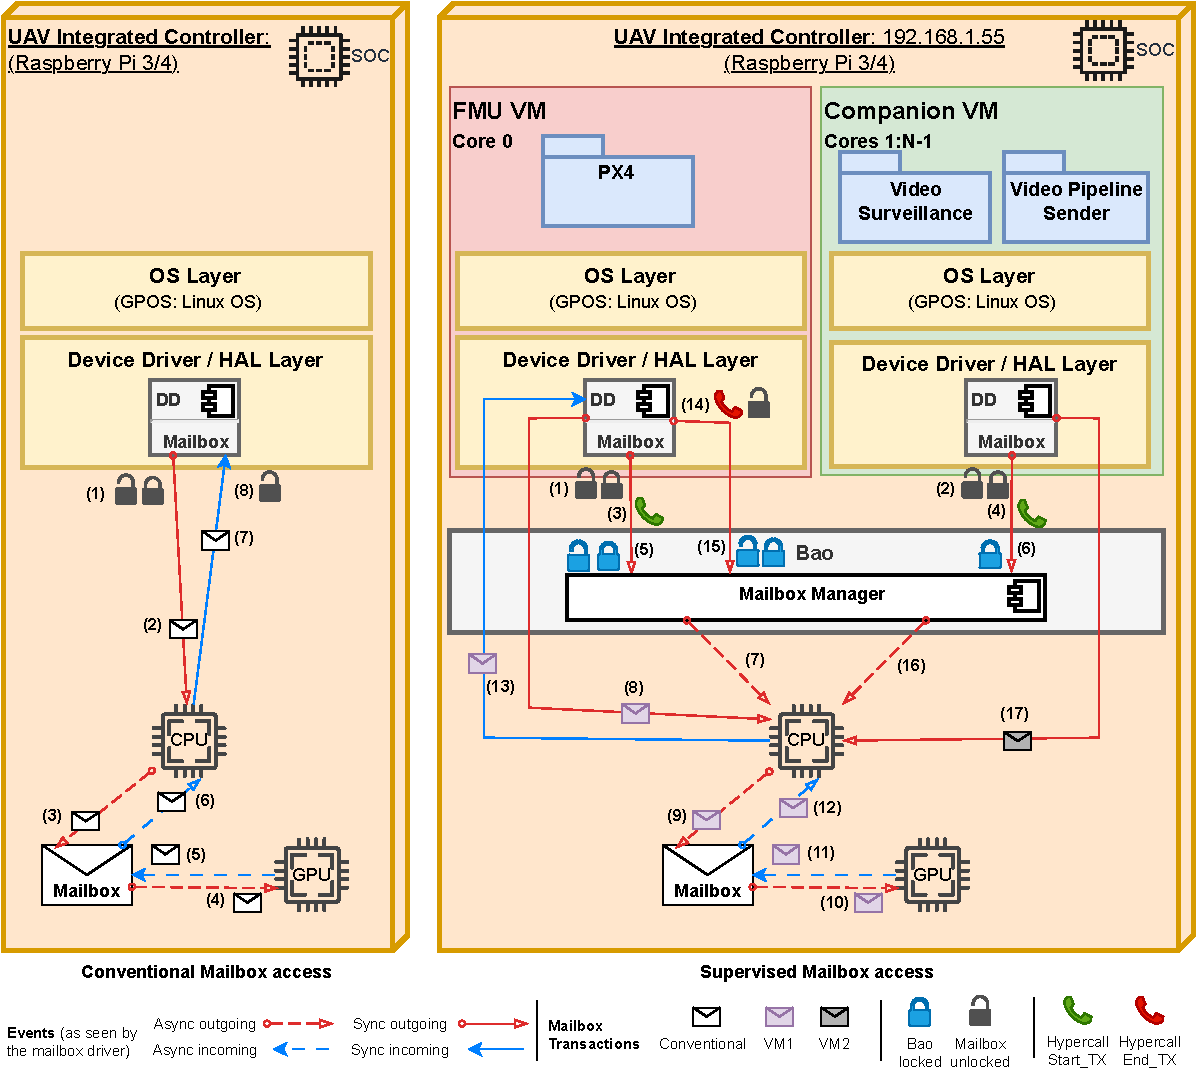
\includegraphics[width=1.0\textwidth]{./img/pdf/uav-main-design-mailbox} 
  \caption{Mailbox access: conventional (left); supervised (right)}%
  \label{fig:design-mailbox}
\end{figure}

The solid lines denote synchronous events, while the dashed lines denote
asynchronous ones.
\textcolor{red}{Red} arrows indicate the outgoing path (from the mailbox
driver), and \textcolor{blue}{blue} arrows indicate the incoming path. Mailbox
transactions are shown as white (conventional), violet (VM1), and grey (VM2)
envelopes. The synchronization mechanisms (locks) appear in brown for the
mailbox and in blue for Bao. Hypercalls are shown as phones: green for
\lstinline{Start_TX} and red for \lstinline{End_TX}. Numbered labels mark the
event sequence in each case.

In the conventional case, the mailbox device driver can initiate a transaction
request if no other is pending (1). The transaction must
be completed (8) before a timeout occurs, freeing the mailbox for further
requests. An interrupt is triggered (2) and the \gls{cpu} forwards the request
to the mailbox (3) which requests data from the \gls{gpu} (4). The \gls{gpu}
firmware handles the transaction and returns a result to the mailbox (5). The
mailbox forwards the response to the mailbox's driver (6, 7) completing
the request and freeing the mailbox~\cite{rpi4-mbox-driver}. 

In the supervised case, VM1's mailbox driver attempts to start a
transaction when none is pending (1). Now,
before transmission, the mailbox driver must signal to Bao it wants
to start a transaction by performing a \lstinline{Start_TX} hypercall (3). Bao
acknowledges this request if no transaction is ongoing, locking the
mailbox manager (5).
VM2 performs the same attempt (2, 4) but must wait because VM1 holds the lock.
%
The mailbox manager handles the hypercall,
associates the guest, target device (mailbox), and interrupt ID, and injects the
interrupt into the appropriate \gls{cpu} (7).
%
VM1's driver issues the transaction to the mailbox (8, 9) which
forwards it to the \gls{gpu} (10).
%
After the \gls{gpu} processes the request, the response returns to the VM1's
driver (11, 12, 13). On completion, VM1 issues \lstinline{End_TX}, signaling Bao
to release the mailbox lock. Bao releases the manager's lock (15), which allows
VM2's pending request (6) to resume. Bao then injects the corresponding
interrupt (16) into the appropriate \gls{cpu}, and VM2's driver proceeds with
its firmware transaction, after which the process repeats itself.

\subsubsection{SSPFS}
\label{sec:final-scenario}
After addressing device sharing between \glspl{vm} via supervised mailbox
management, we assigned hardware resources to each \gls{vm}.
%
Fig.~\ref{fig:hw-map-2} and Fig.~\ref{fig:hw-map-3} show the device trees
for the PX4 \gls{vm} and Companion \gls{vm}, respectively.

\begin{figure}[!hbt]
  \centering
  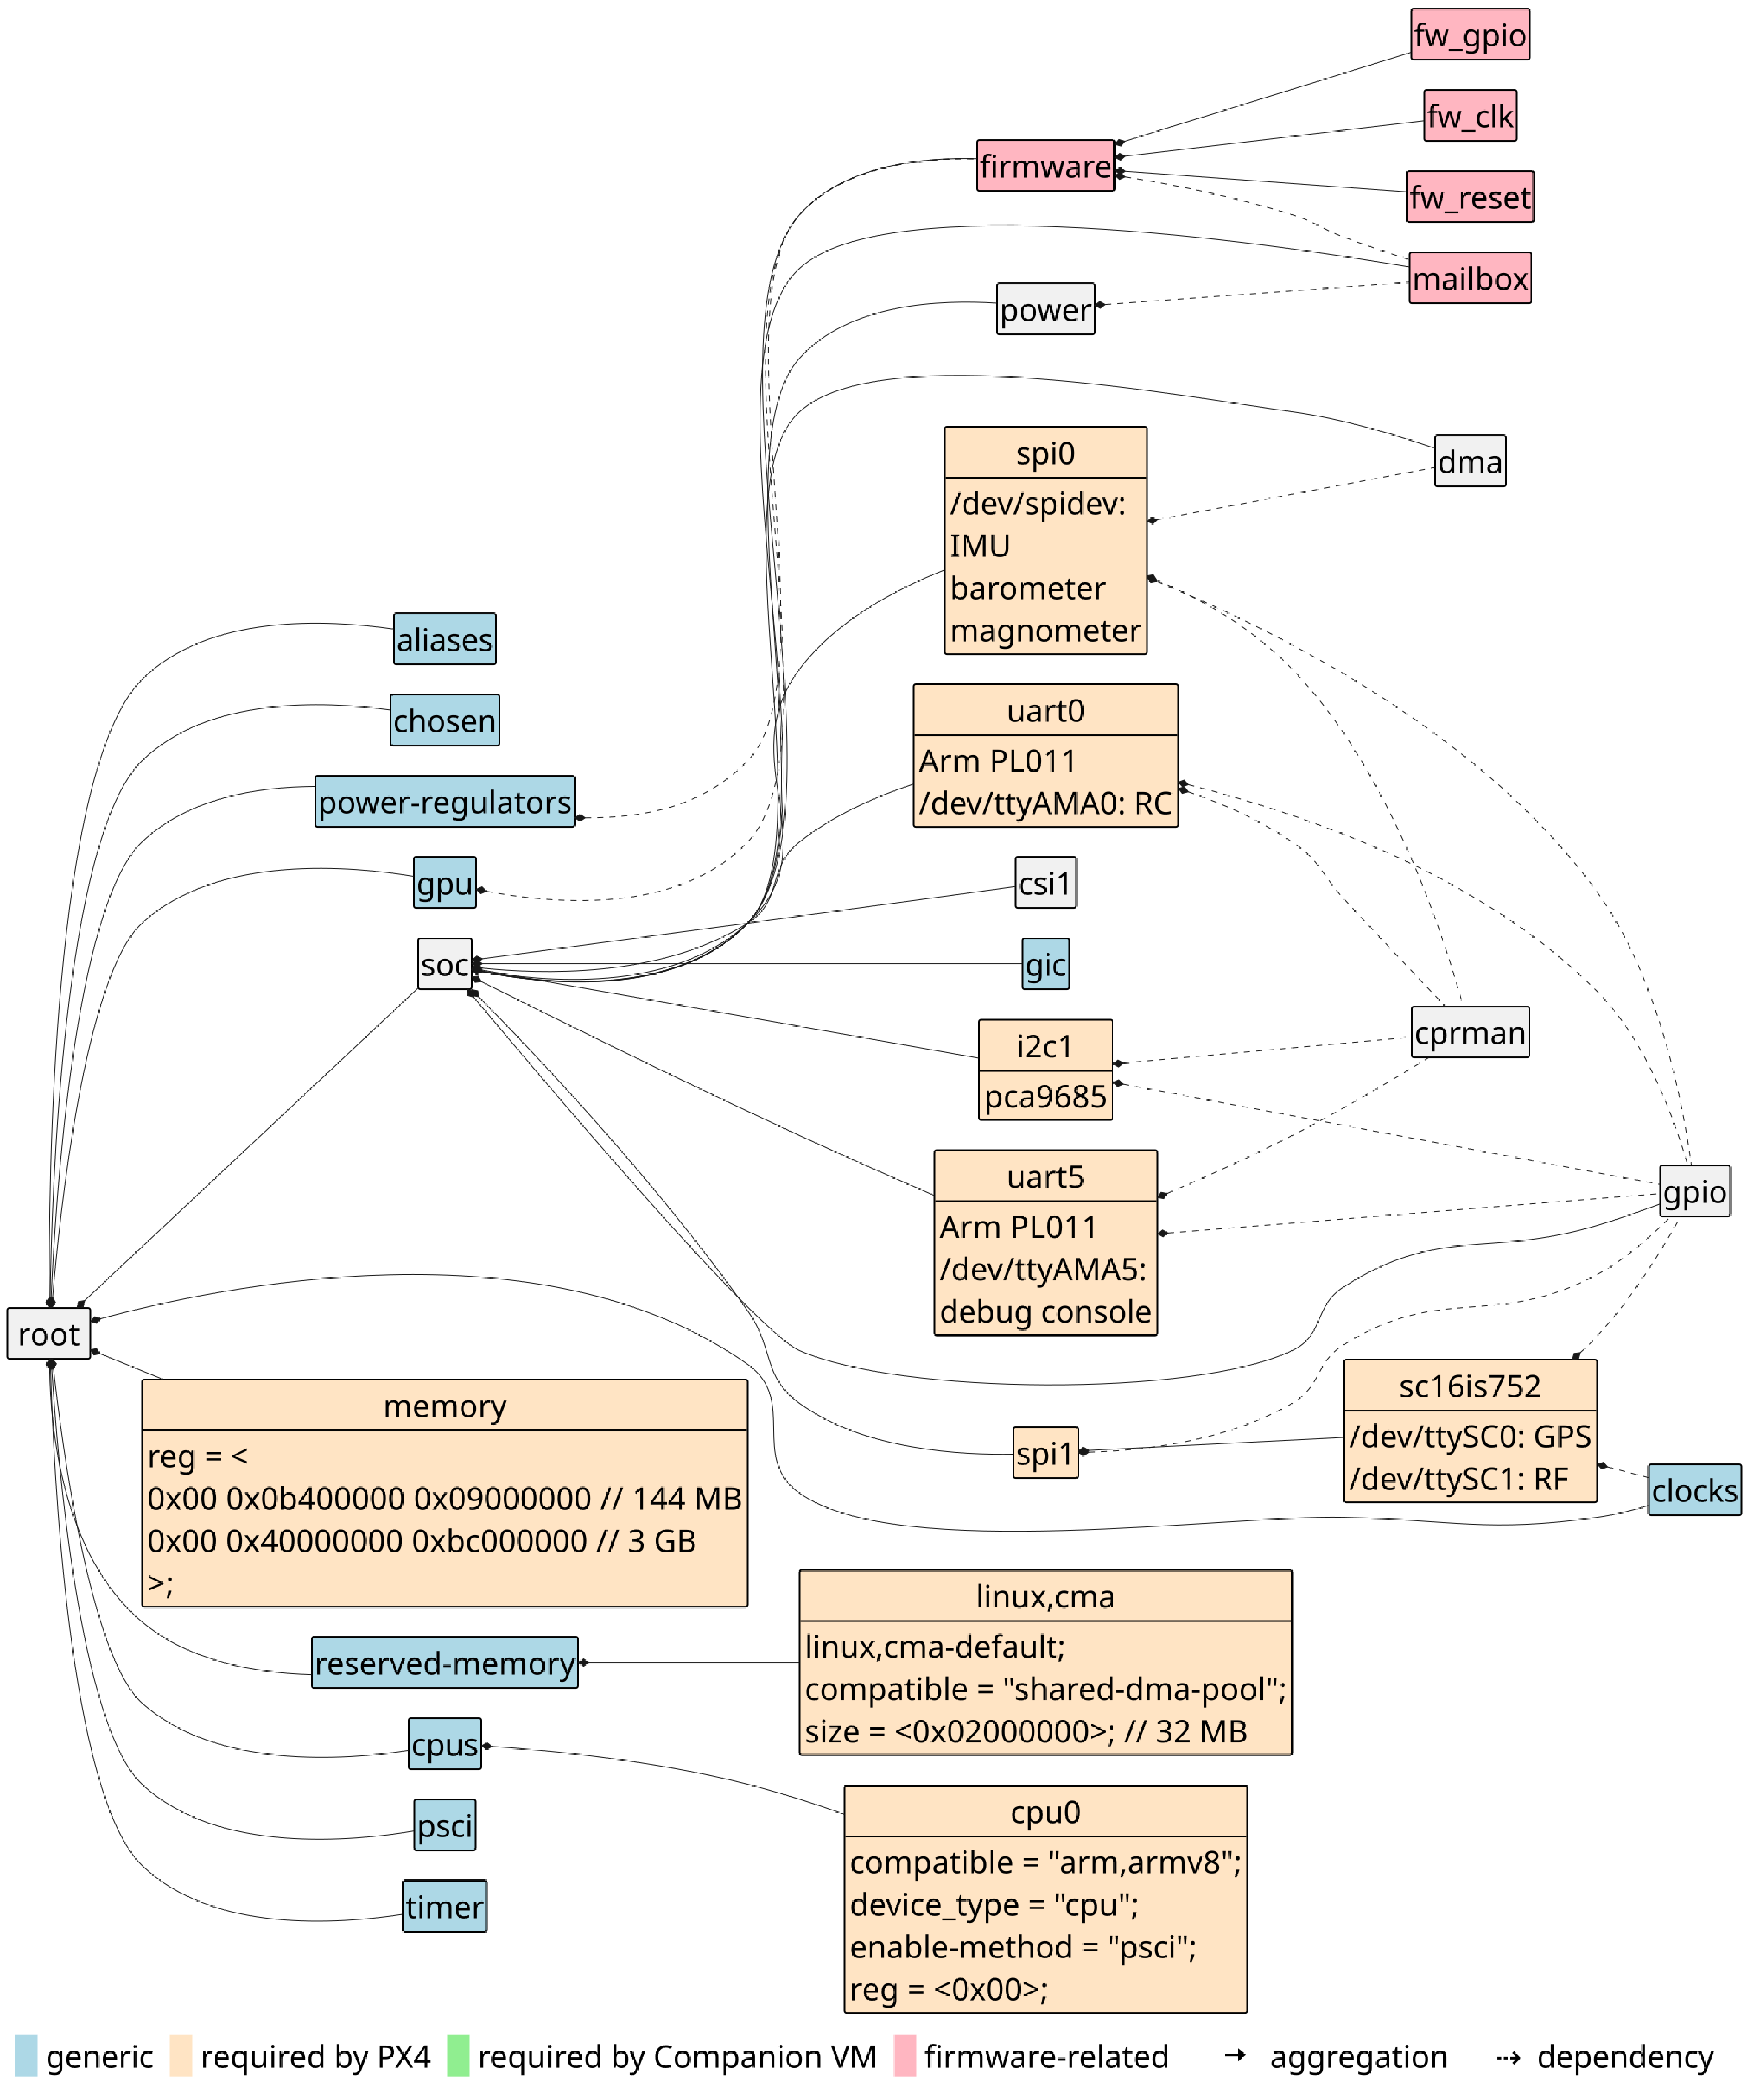
\includegraphics[width=0.85\textwidth]{./img/pdf/hw-map-2} 
  \caption[Hardware mapping: SSPFS device tree -- PX4]{Hardware mapping:
  \gls{sspfs} device tree -- PX4}%
  \label{fig:hw-map-2}
\end{figure}

\begin{figure}[!hbt]
  \centering
  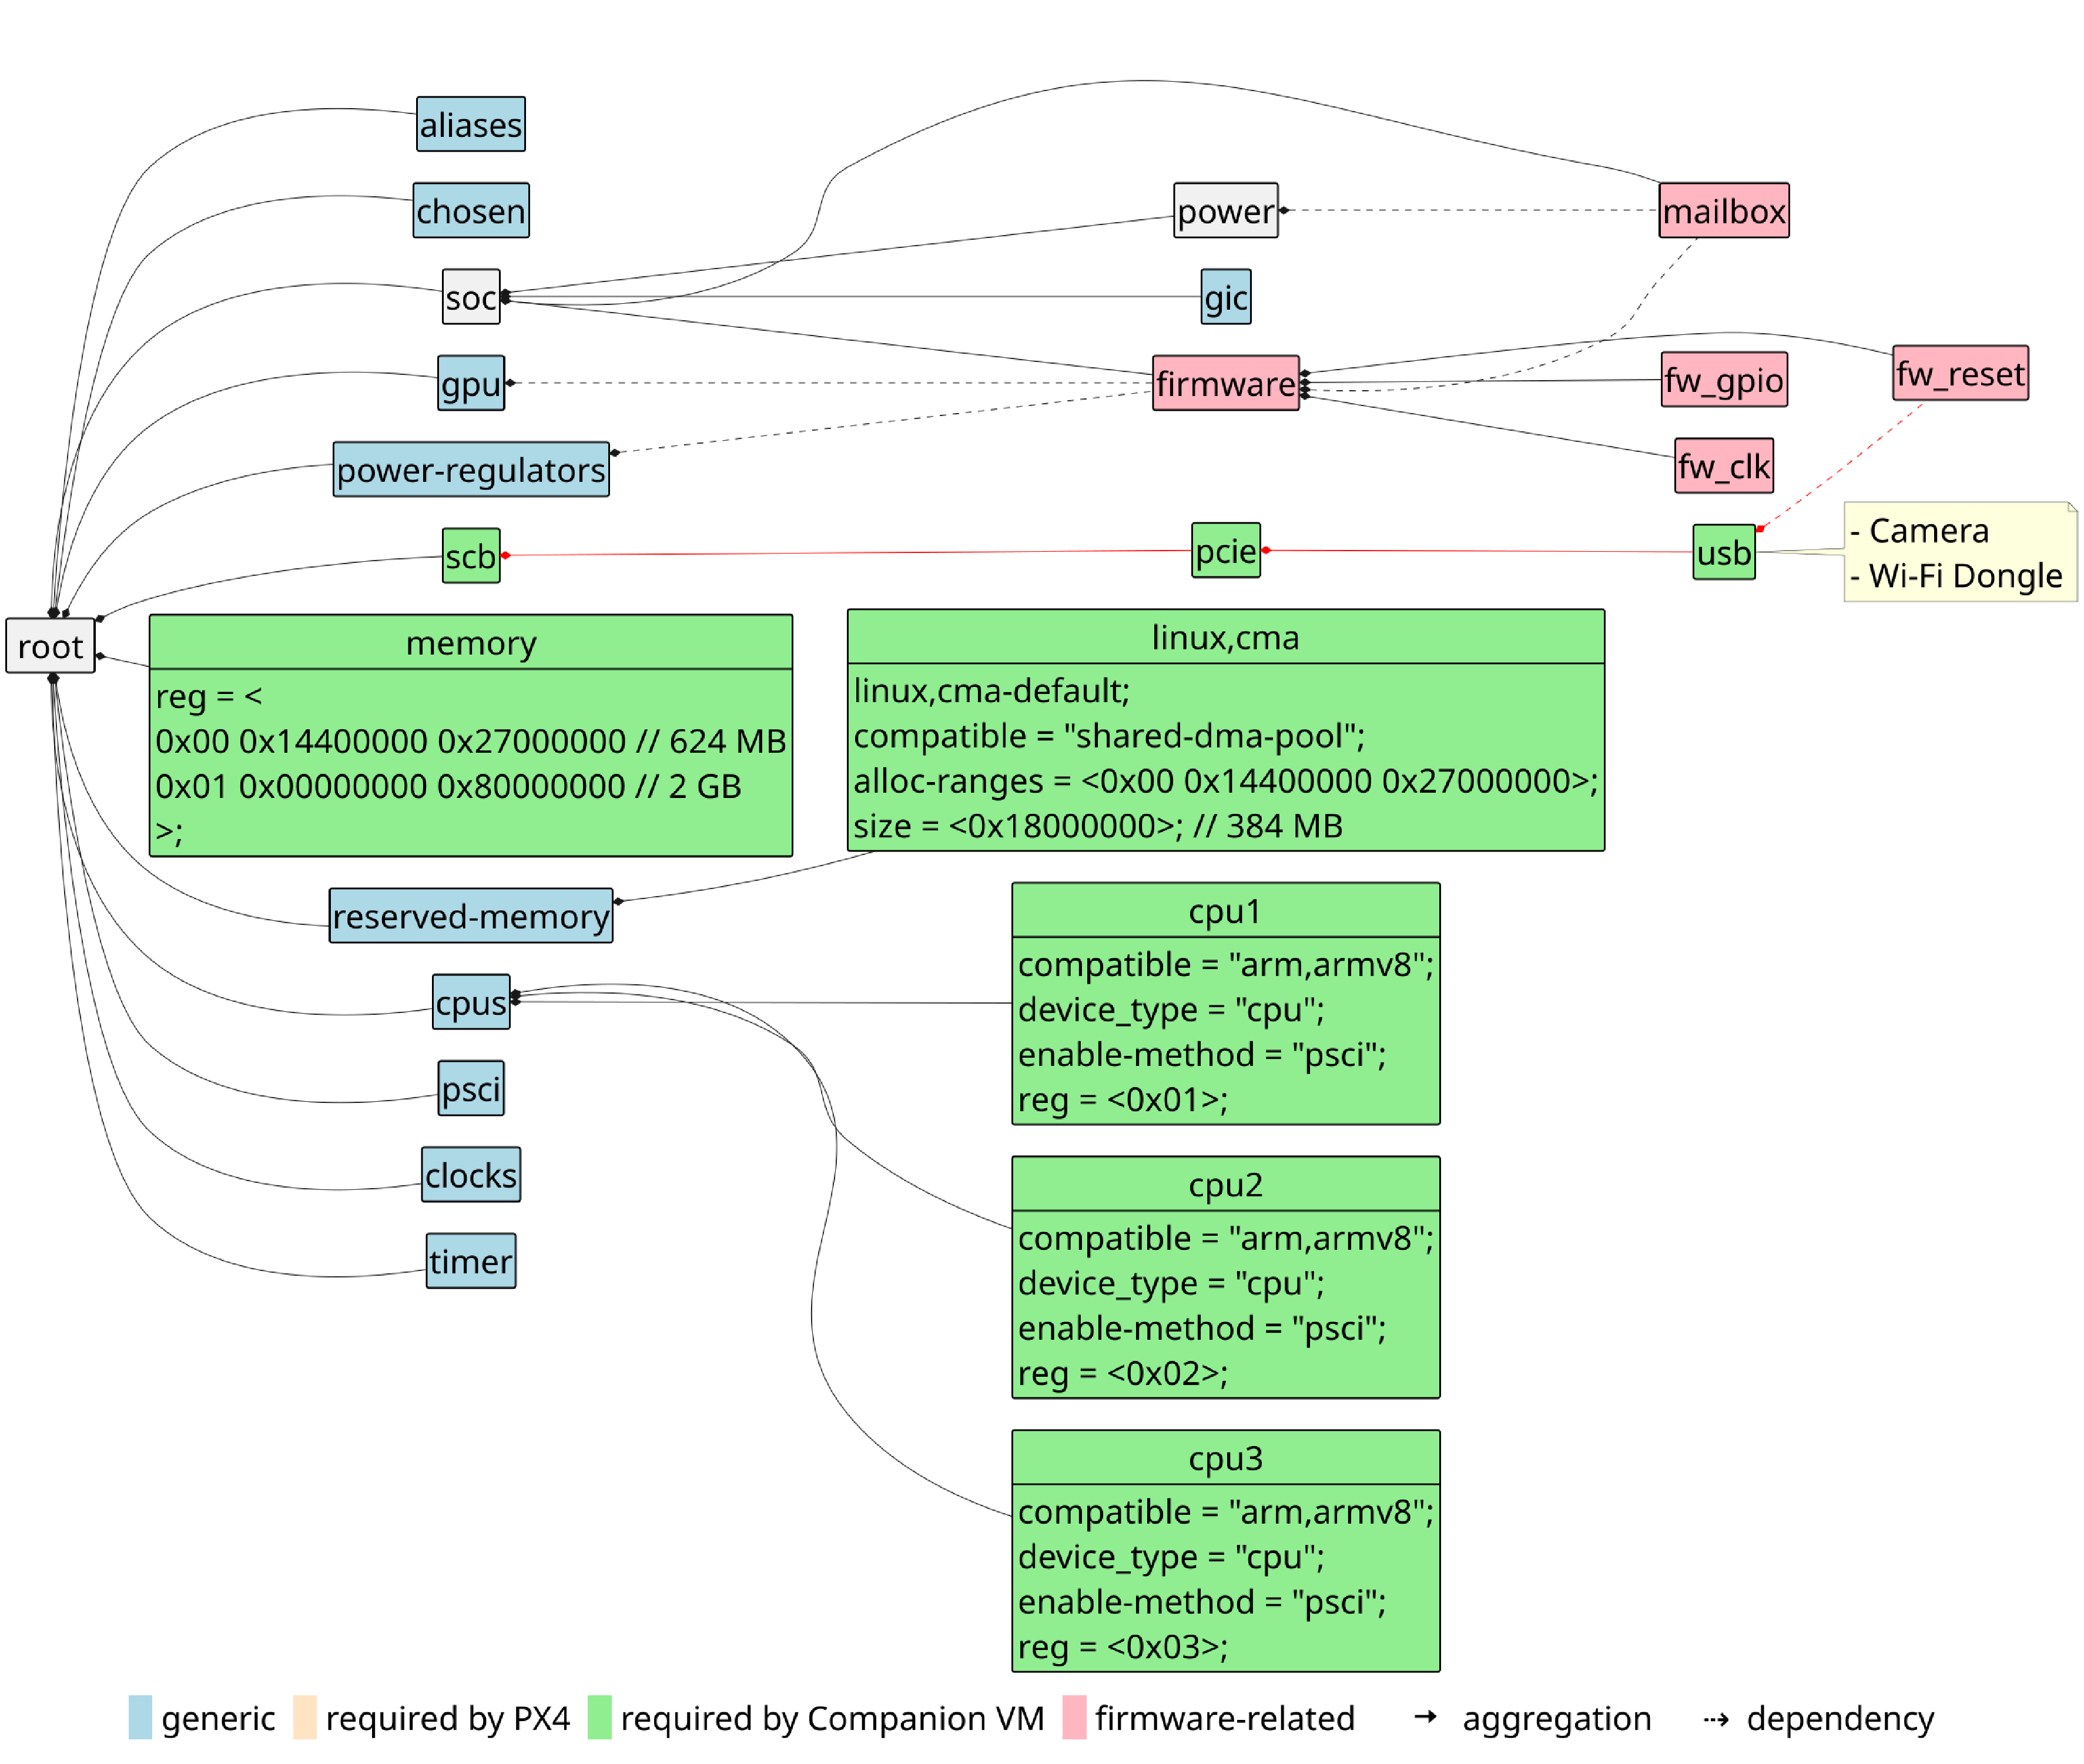
\includegraphics[width=0.85\textwidth]{./img/pdf/hw-map-3} 
  \caption[Hardware mapping: SSPFS device tree -- Companion VM]{Hardware
    mapping: \gls{sspfs} device tree -- Companion VM}%
  \label{fig:hw-map-3}
\end{figure}

%
The PX4 \gls{vm} includes only essential onboard
sensors/actuators and an optional debug console.
Memory is split into two \gls{ram} regions of 144 MB and 3 GB, respectively. Within the first region, a 32 MB
\gls{cma} region is reserved to support \gls{dma} transactions for \gls{spi}
devices, which operate exclusively within the first 1 GB of
memory~\cite{bcm2711peripherals}. Processing resources include a single Arm A72
\gls{cpu} (core 0).
%
The Companion \gls{vm} exposes the \gls{usb} interface for a \gls{usb} camera and Wi-Fi dongle. Memory allocation features two
\gls{ram} regions of 624 MB and 2 GB, respectively. Within the first region, a
384 MB \gls{cma} region supports video pipeline operations, also restricted to the first 1
GB of memory~\cite{bcm2711peripherals}. Processing resources include three Arm
A72 \glspl{cpu} (cores 1--3).

\subsection{Addons}
\label{sec:addons}
The Companion \gls{vm} requires two \gls{usb} devices: a camera and a Wi-Fi
dongle. Fig.~\ref{fig:addons-cam} shows the selected camera, the Creative Live!
Cam Sync 1080p V2~\cite{creative-cam}. It is an affordable \gls{usb} device
supporting full~\gls{hd} capture  (1920×1080 @ 30\gls{fps}) with dual built-in
microphones. It is plug-and-play on Linux with in-kernel driver support, and its
long cable allows flexible placement on the \gls{uav}.

Fig.~\ref{fig:addons-wifi} shows the selected \gls{usb} Wi-Fi dongle, the EDUP
AX3000. This dual high-gain antenna model offers tri-band support (2.4, 5, and
6~GHz) and data rates up to 3000~\gls{mbps} over a \gls{usb}~3.0 interface~\cite{ax3000-specs}. It uses the Mediatek \lstinline{mt7921au} chipset
with broad \gls{os} compatibility and has been supported in-kernel since
Linux~5.18~\cite{ax3000-linux}.

% The Companion \gls{vm} requires two \gls{usb} devices: a camera and Wi-Fi
% dongle. Fig.~\ref{fig:addons-cam} presents the selected \gls{usb} camera -- the
% Creative Live! Cam Sync 1080p V2~\cite{creative-cam}.
% %
% It is an affordable \gls{usb} camera with full
% \gls{hd} video capture (1920x1080 @ 30 \gls{fps}) and dual built-in
% microphone. This camera is a plug-and-play device with built-in drivers for
% Linux available out of the box. Lastly, due to its long cable it can be
% positioned freely in the \gls{uav}. 
% %
% Fig.~\ref{fig:addons-wifi} presents the selected \gls{usb} Wi-Fi dongle --- the
% EDUP AX3000. This dual high-gain antena device has tri-band support --- 2.4 GHz, 5, and 6
% GHz --- and it can achieve data transfer rates
% of up to 3000 \gls{mbps} on the \gls{usb} 3.0 interface~\cite{ax3000-specs}. It contains a Mediatek
% \lstinline{mt7921au} chipset with a wide \gls{os} compatibility, supported
% in-kernel since Linux kernel 5.18~\cite{ax3000-linux}.

\begin{figure}[!hbt]
  \centering
  % Row 1: Two half-width images
  \begin{subfigure}[t]{0.49\textwidth}
    \centering
    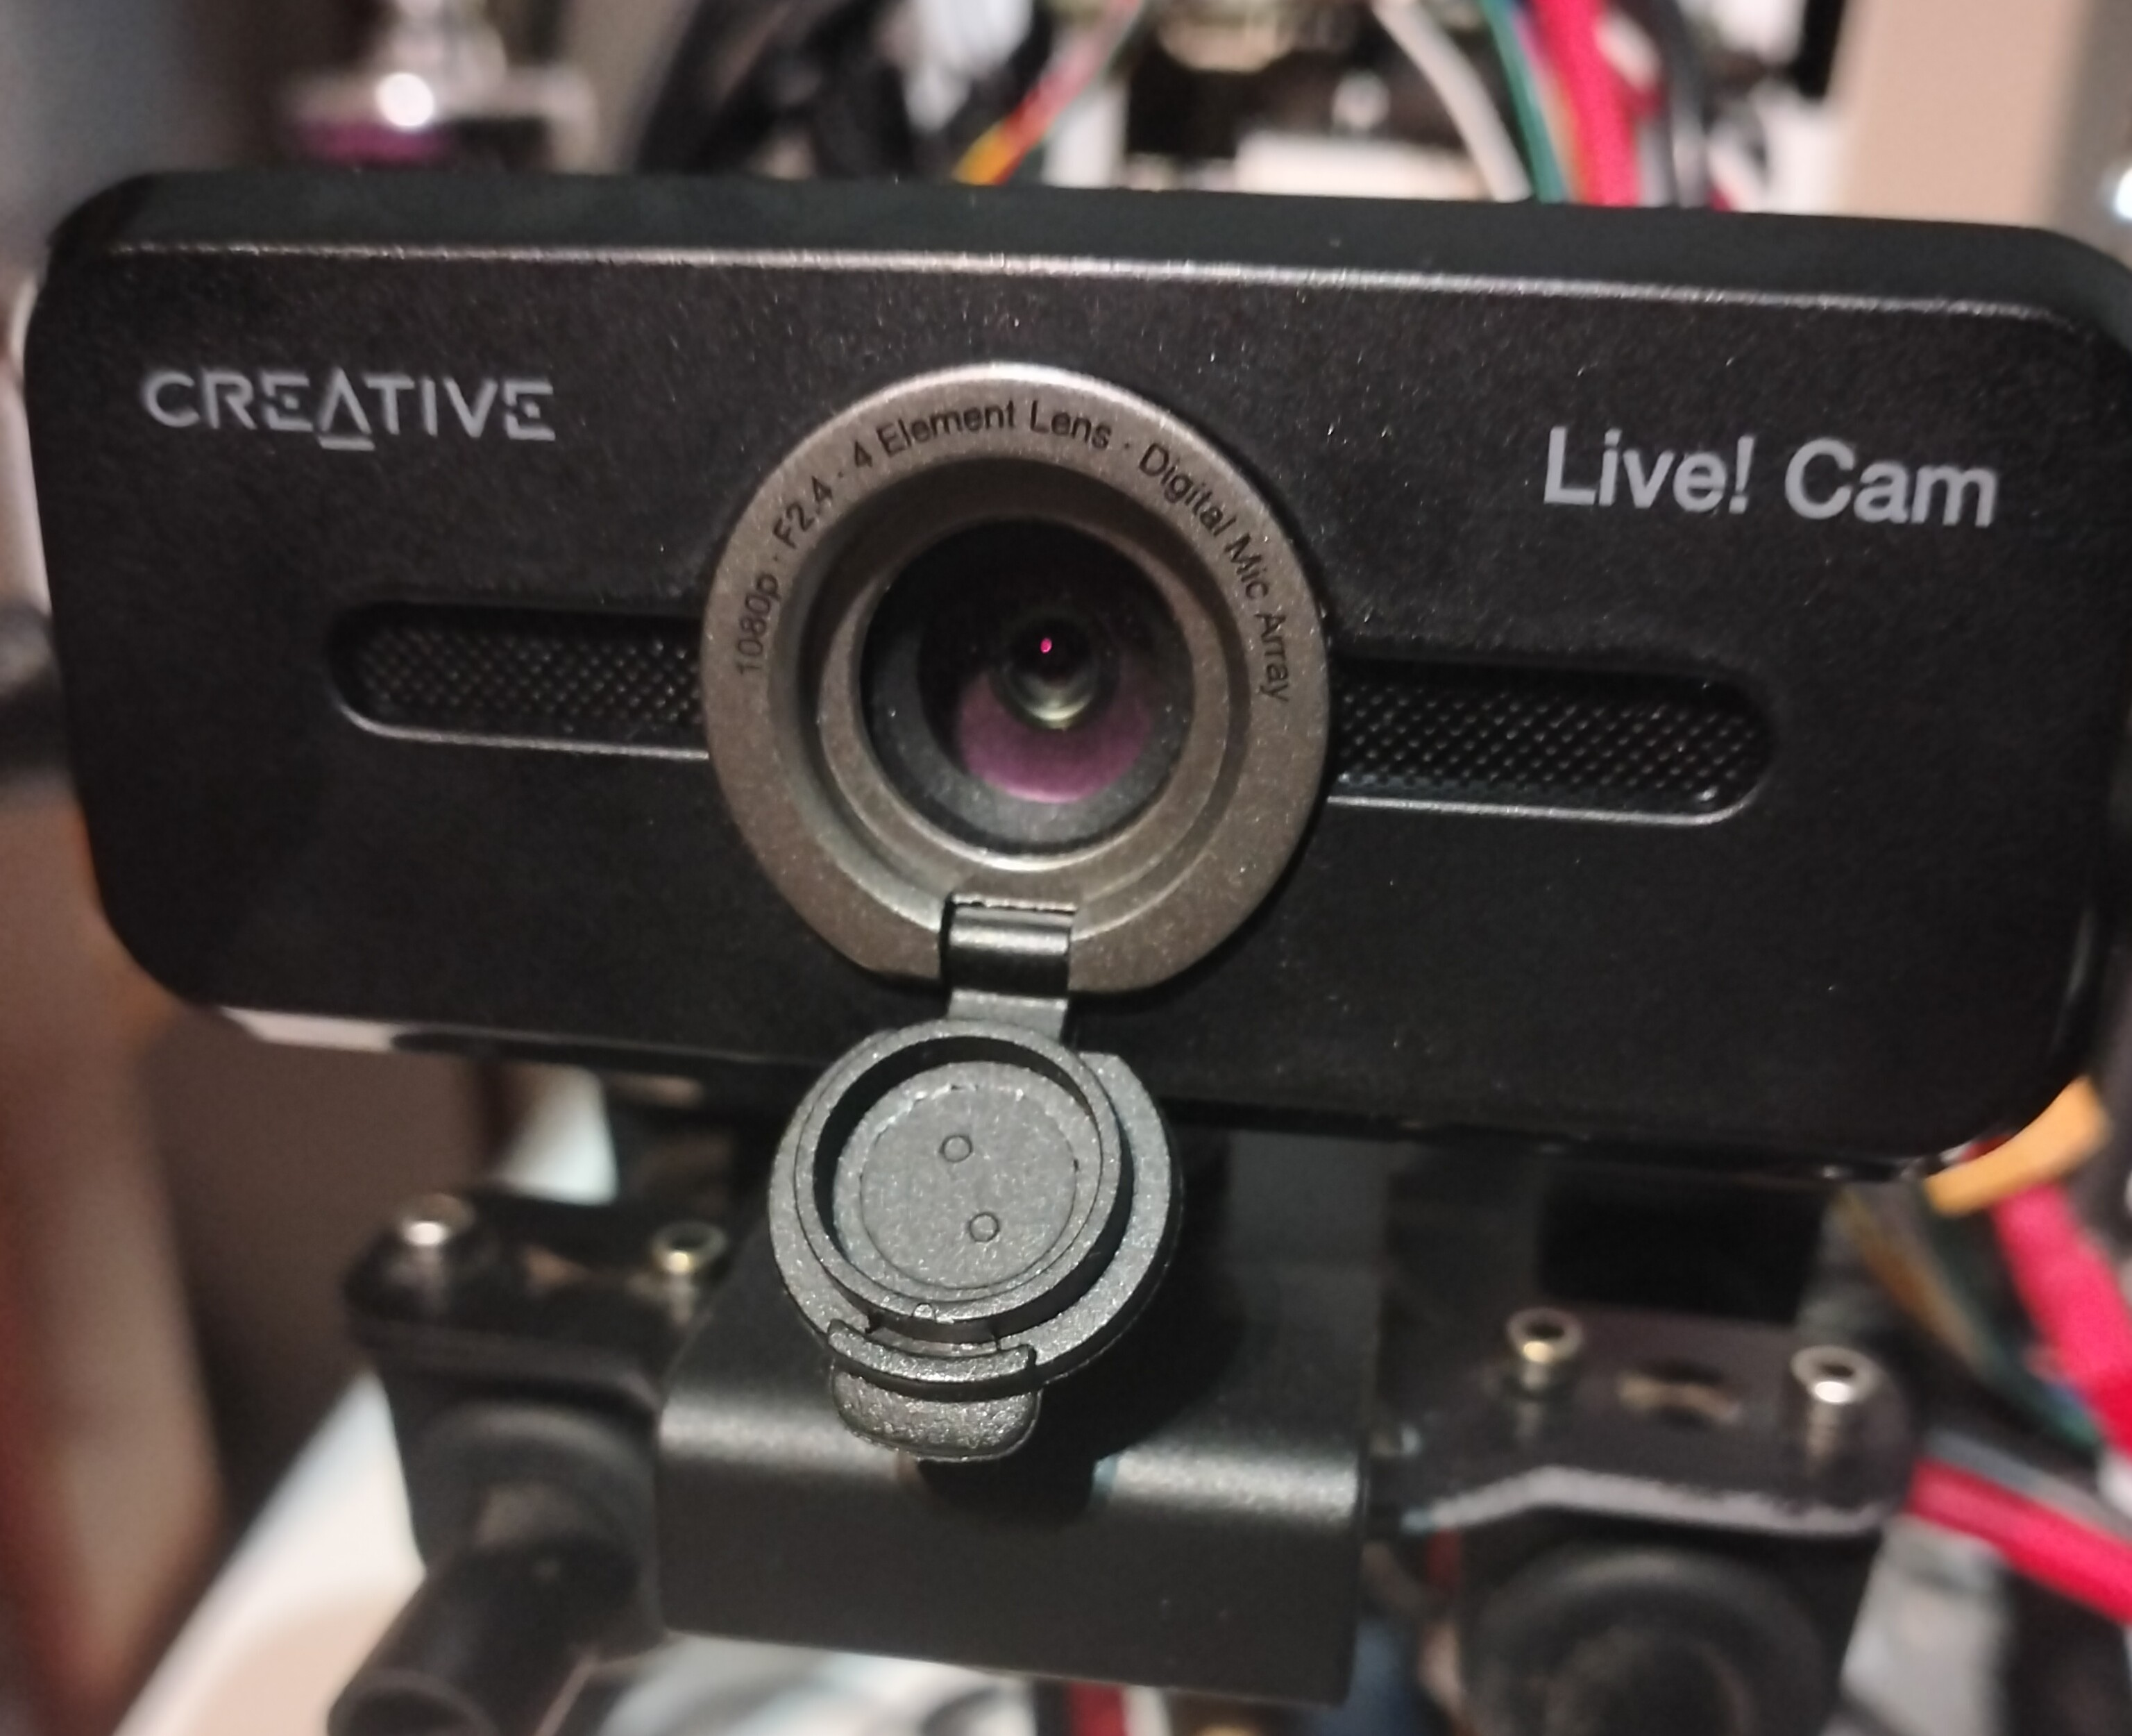
\includegraphics[width=1.0\textwidth]{./img/jpg/creative-cam} 
    \caption{USB Camera -- Creative Live!}%
    \label{fig:addons-cam}
  \end{subfigure}
%  \\[0.5\baselineskip] % Vertical space after first row
  \begin{subfigure}[t]{0.49\textwidth}
    \centering
  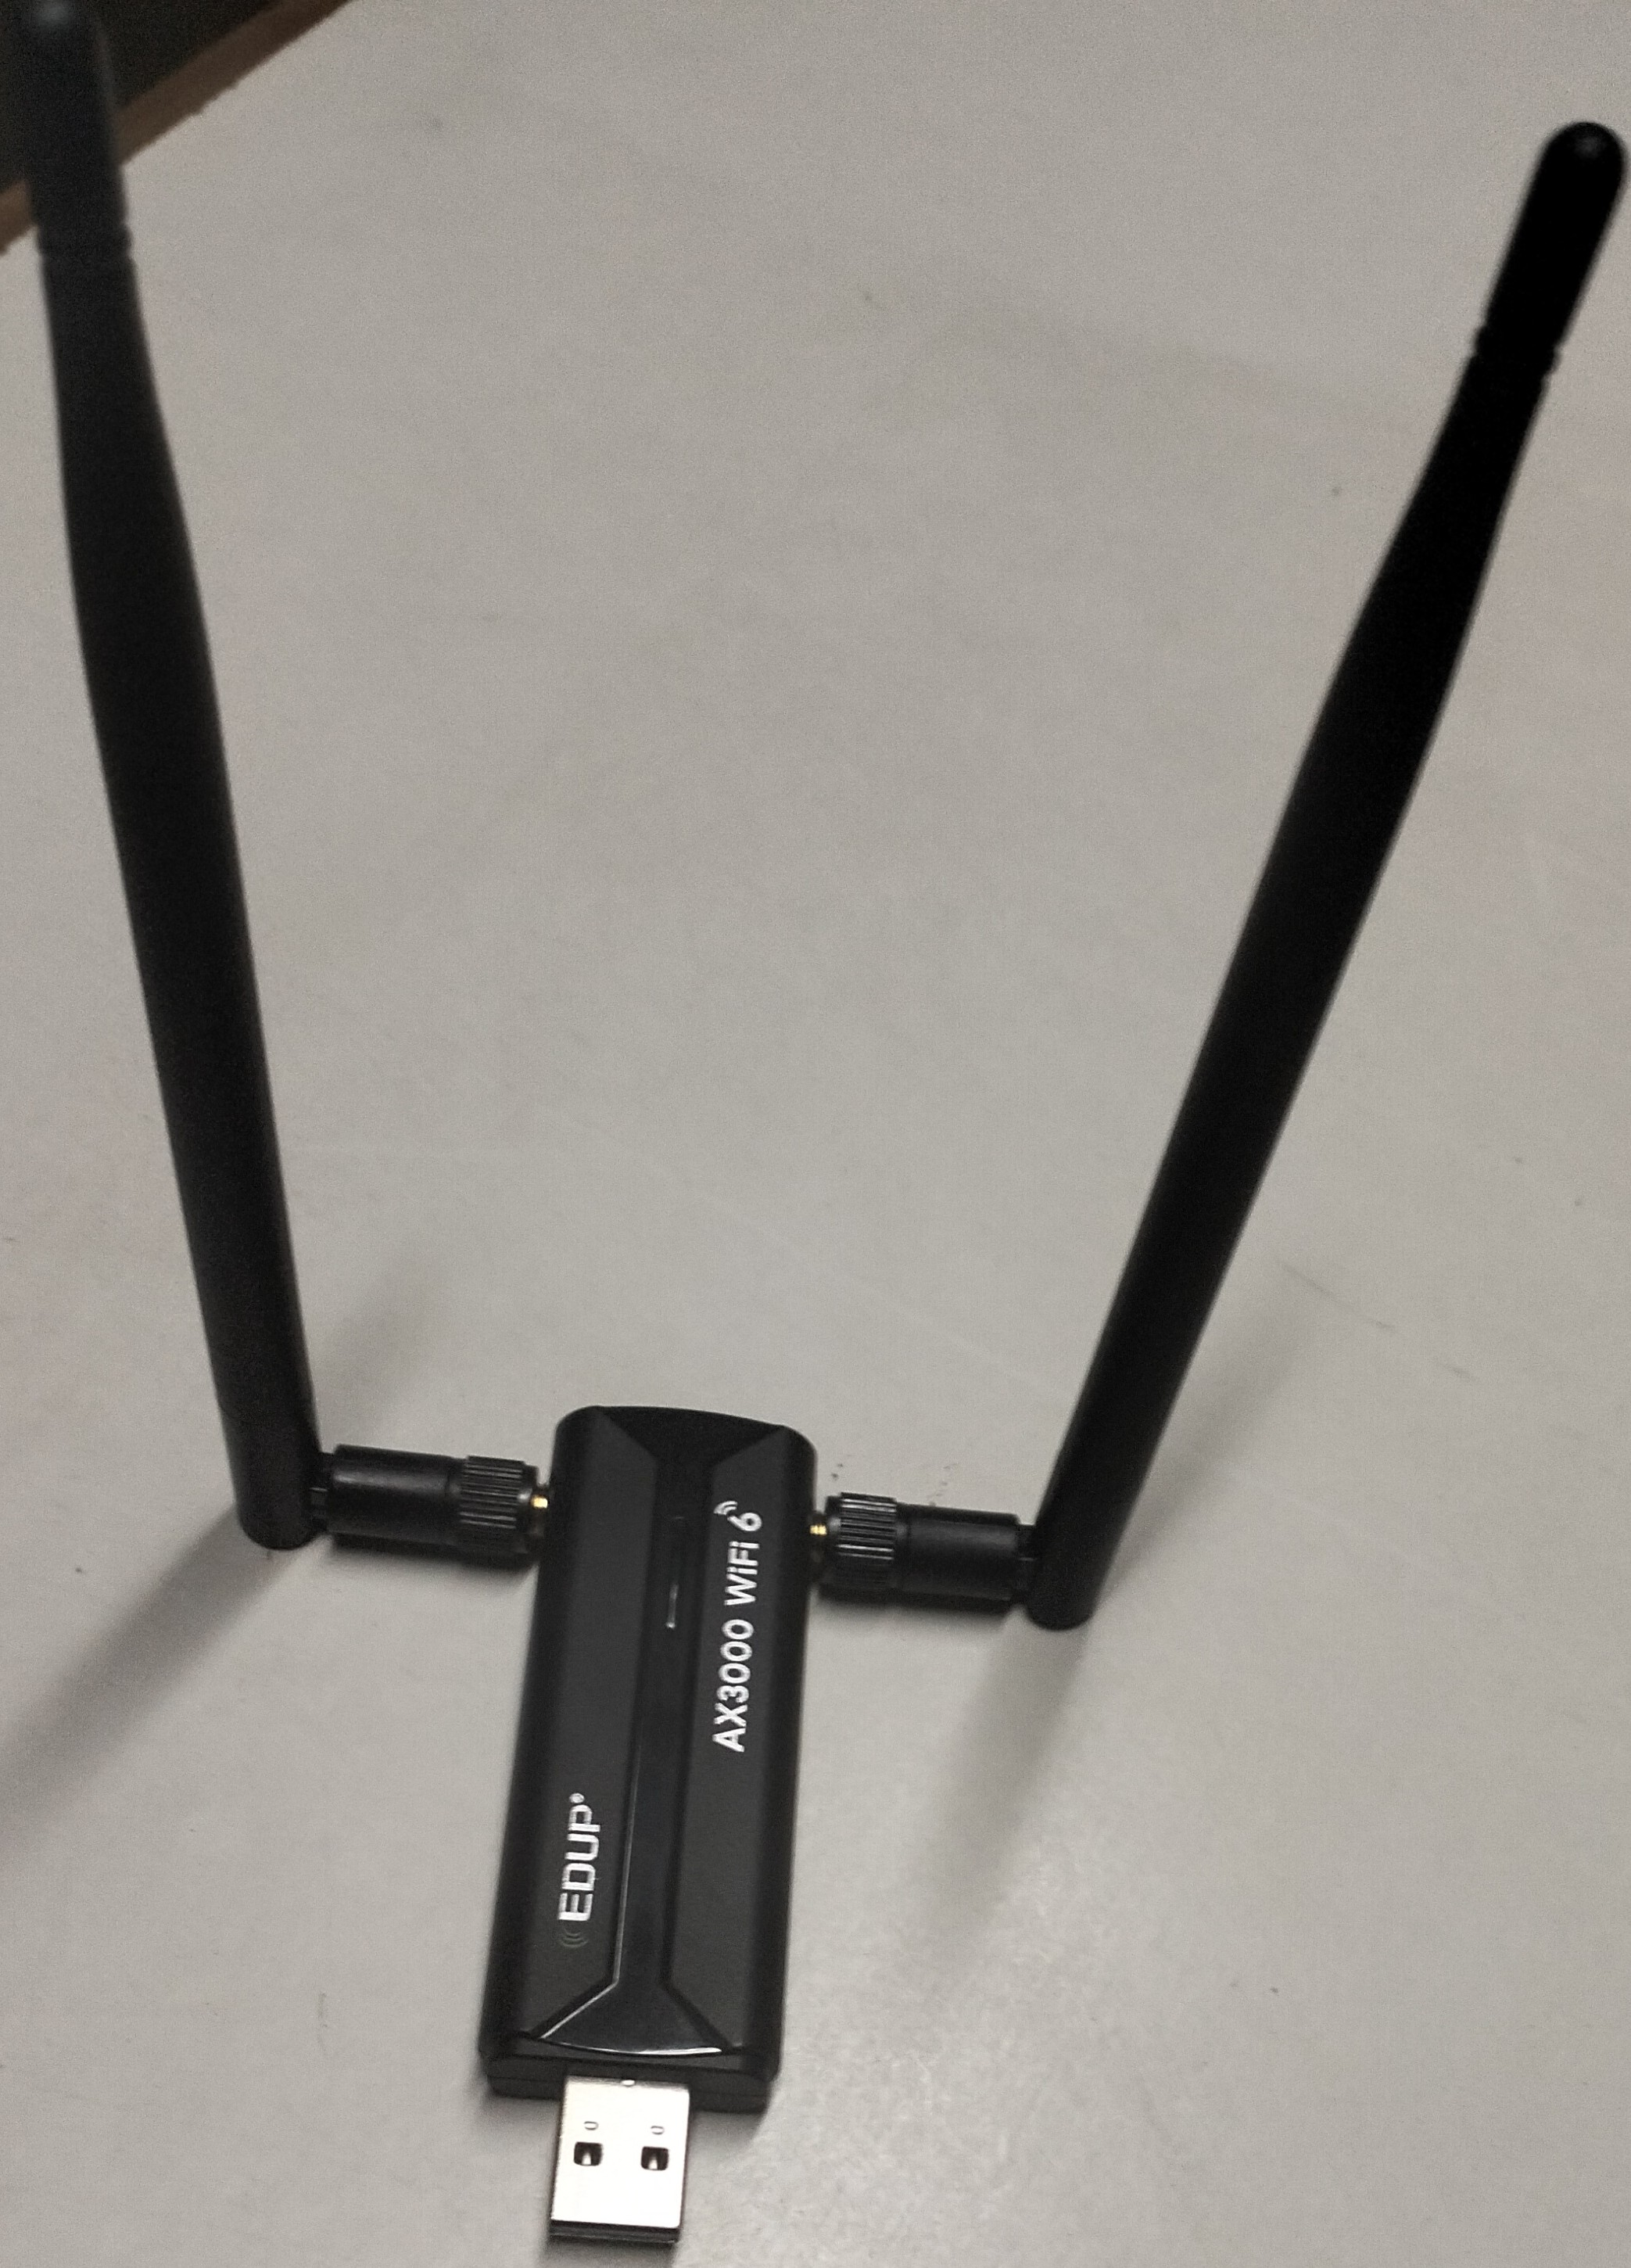
\includegraphics[width=0.6\textwidth]{./img/jpg/ax3000} 
    \caption{USB Wi-Fi dongle -- EDUP AX3000}%
    \label{fig:addons-wifi}
  \end{subfigure}
  \caption{Addons}
  \label{fig:addons}
\end{figure}

% \begin{figure}[!hbt]
%   \centering
%   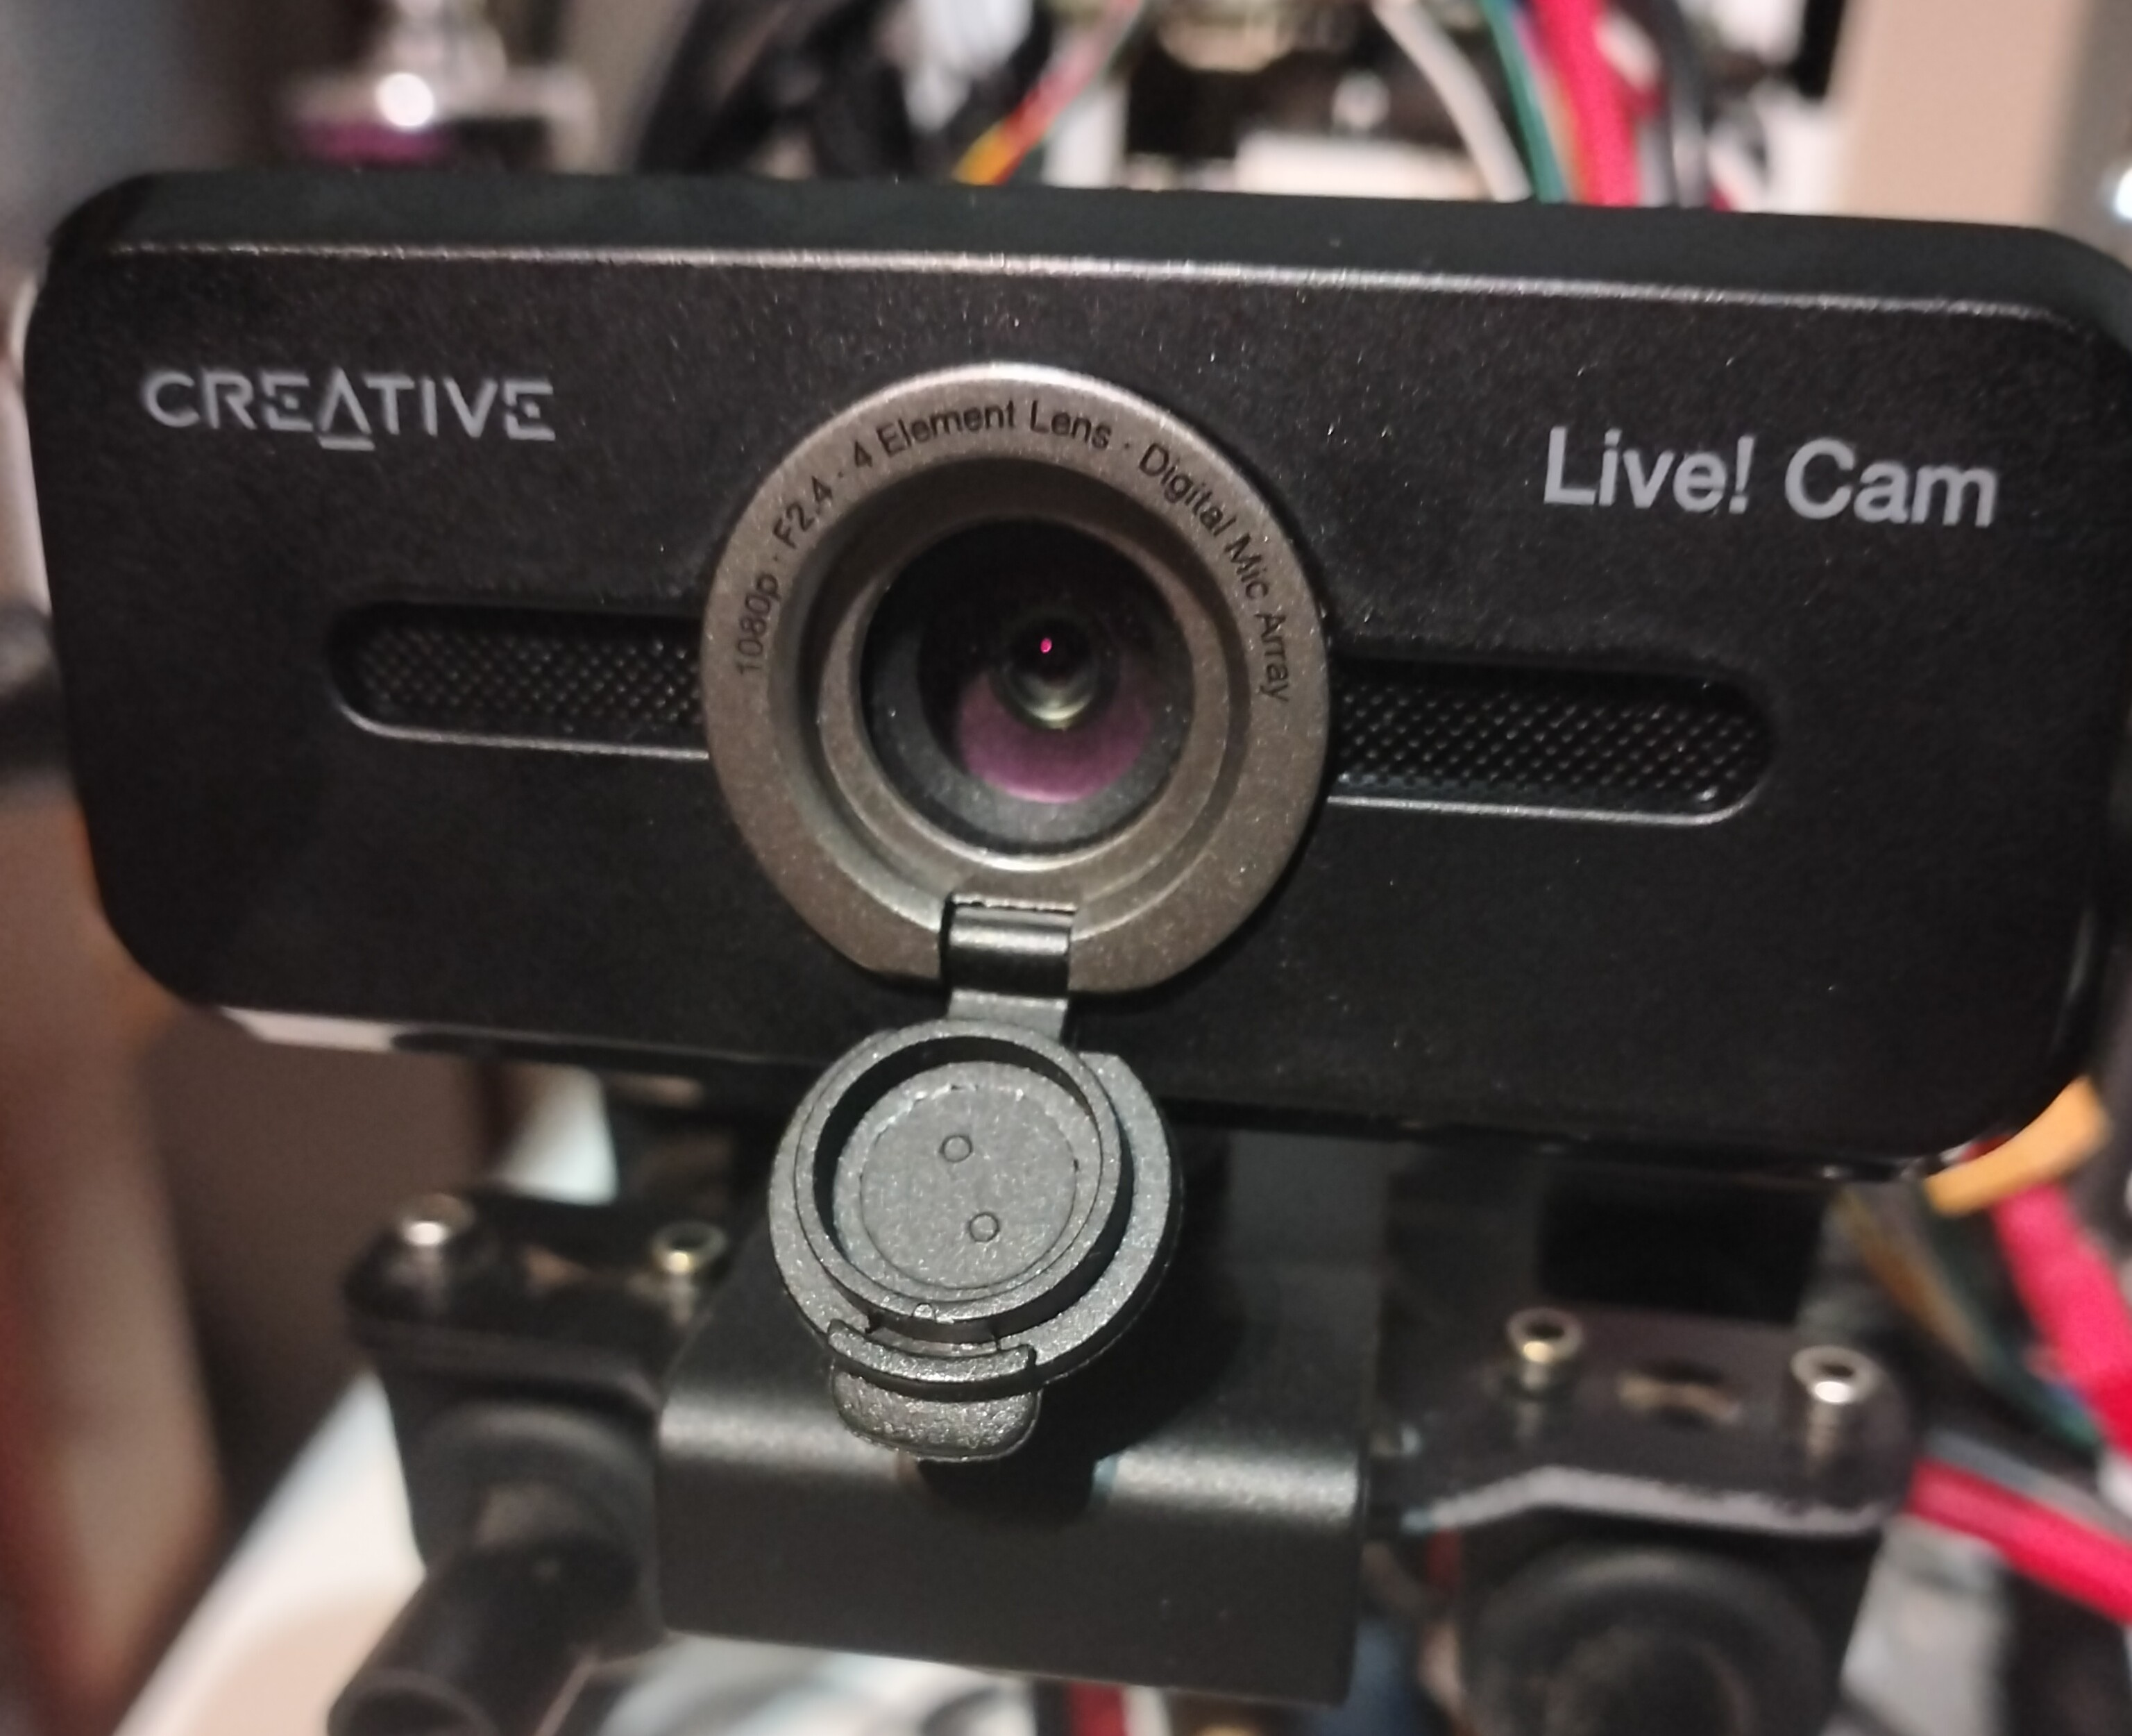
\includegraphics[width=0.4\textwidth]{./img/jpg/creative-cam} 
%   \caption{Addons: USB Creative Camera}%
%   \label{fig:usb-cam}
% \end{figure}

% \begin{figure}[!hbt]
%   \centering
%   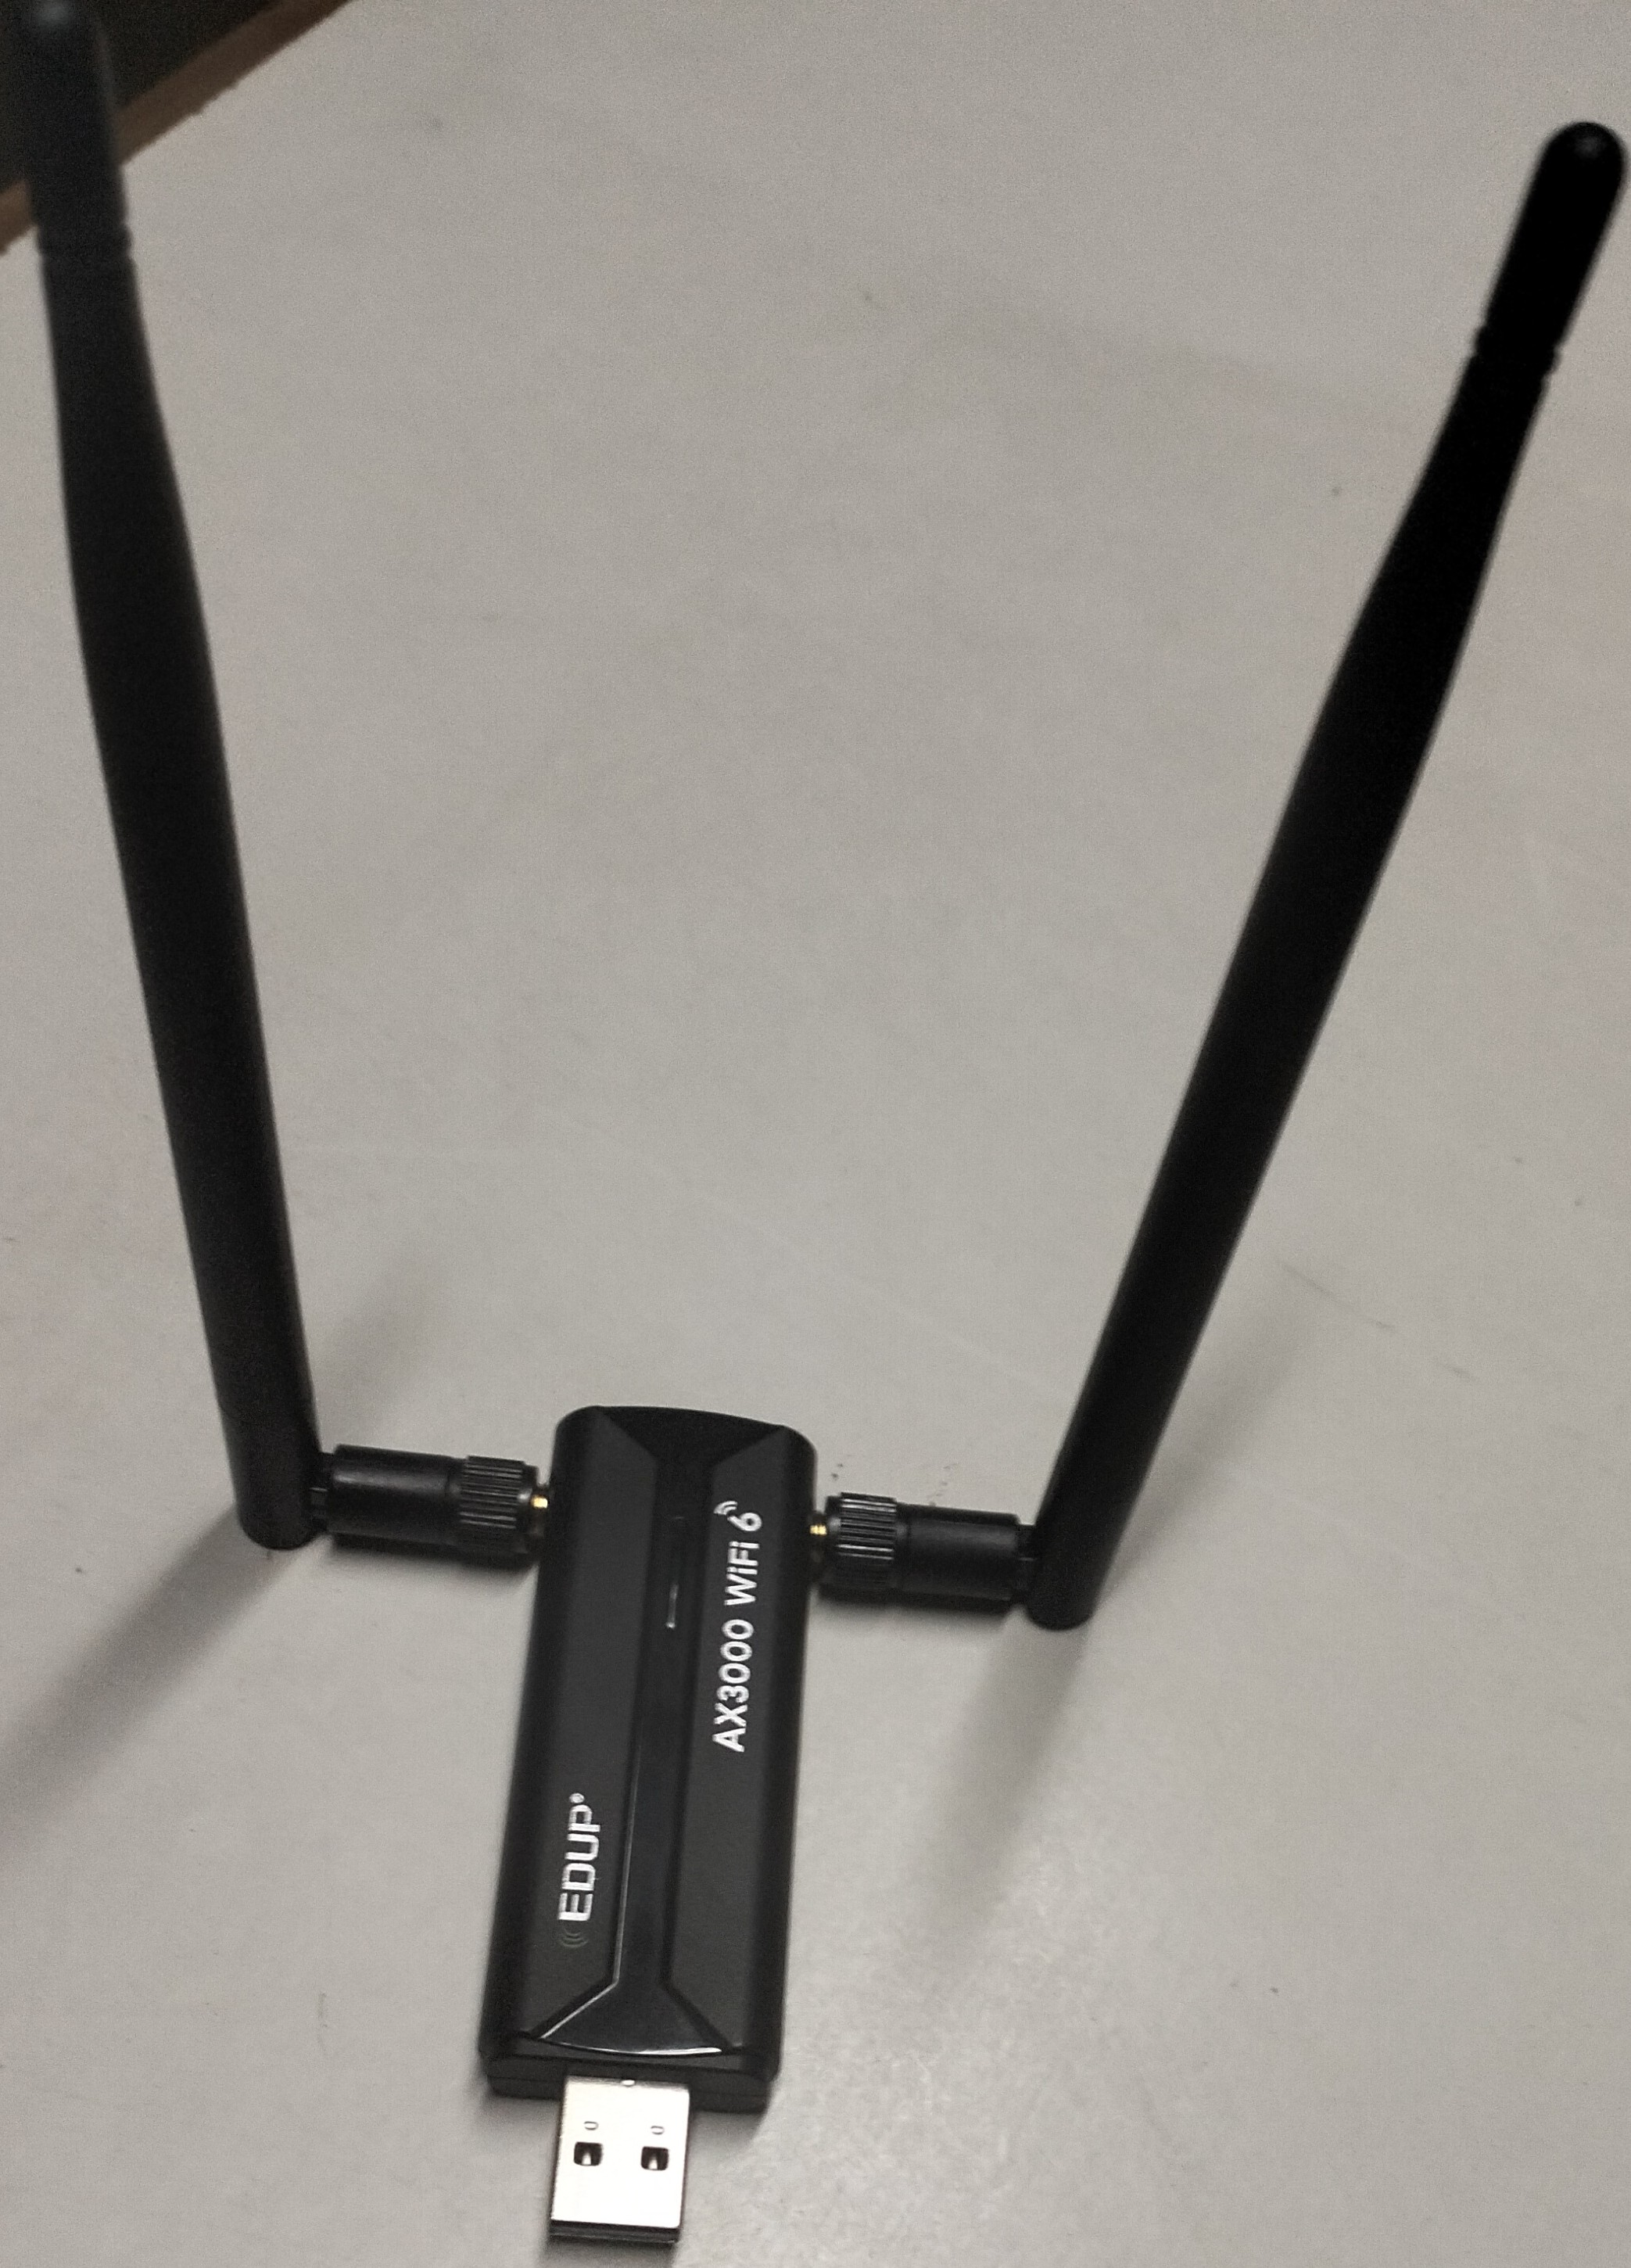
\includegraphics[width=0.4\textwidth]{./img/jpg/ax3000} 
%   \caption{Addons: USB Wi-Fi dongle --- EDUP AX3000}%
%   \label{fig:usb-wifi}
% \end{figure}

% \section{Summary}
% \label{sec:summary}
% Conventional flight stacks address mixed-criticality through multi-platform designs, increasing UAV weight and footprint. Platform integration represents a key design objective, but requires appropriate supervision to be viable.

% This chapter presented three solutions for PX4-based video surveillance applications: conventional (unsupervised multi-platform), unsupervised single-platform (\gls{uspfs}), and supervised single-platform (\gls{sspfs}). The conventional approach established the foundation for platform integration. Subsequent consolidation merged flight controller and companion computer functions into the \gls{uspfs} architecture using a Raspberry Pi 4 with Pilot Pi shield. However, the \gls{uspfs} provides no isolation between systems, allowing failures in non-critical components to propagate to the \gls{fmu}. Platform consolidation with system isolation was therefore achieved through Bao hypervisor supervision, forming the \gls{sspfs} solution.

% Bao's static partitioning requirement creates potential hardware resource conflicts between \glspl{vm}. This challenge was addressed through \gls{uavic} hardware selection and mapping, producing solution-specific device trees. Identified conflicts were resolved by assigning \gls{usb} devices (camera and Wi-Fi dongle) to the companion computer \gls{vm}. One critical shared dependency remained—the firmware mailbox required for Arm \gls{cpu}-\gls{gpu} communication. A mailbox access supervision mechanism was consequently developed for Bao, enabling both \glspl{vm} to communicate securely with the board's firmware.


%%% Local Variables:
%%% mode: latex
%%% TeX-master: "../template"
%%% reftex-default-bibliography: ("../Bibliography/mieeic.bib")
%%% ispell-local-dictionary: "american"
%%% End:
